%Experimental Apparatus
\label{ch:Experimental_Apparatus}

\section{The LHC}
\label{the_lhc}

The Large Hadron Collider (LHC)~\cite{Brüning:782076} at CERN is currently the world's largest and most powerful hadron accelerator and collider.
It is located in a circular tunnel roughly 100 m beneath the borders of Switzerland and France. The tunnel is about 27 kilometers long and was initially built for the Large Electron-Positron Collider (LEP), which operated from 1989 to 2000. Construction of the LHC began in 1998 and was completed in 2008. There are eight Interaction Points (IP) where particle beams can collide, four located in caverns, each housing one of the four experiments of the LHC: ATLAS~\cite{TheATLASCollaboration_2008}, CMS~\cite{TheCMSCollaboration_2008}, LHCb~\cite{TheLHCbCollaboration_2008}, and ALICE~\cite{TheALICECollaboration_2008}.
The ATLAS and CMS experiments search for the same types of collision events and are used to cross-check one another’s results.

The LHC was designed to collide proton beams at a center-of-mass energy of 14 TeV and a maximum instantaneous luminosity of 
$10 \, \mathrm{nb}^{-1} \, \mathrm{s}^{-1} (10^{34} \, \mathrm{cm}^{-2}\mathrm{s}^{-1})$~\cite{LyndonEvans_2008}.
The proton beams are guided by a sophisticated system of superconducting magnets. This system includes 1,232 dipole magnets with an \SI{8.3}{\tesla} strength for bending the beams and 392 main quadrupole magnets with a \SI{7.5}{\tesla} strength for focusing the beams~\cite{1288863}~\cite{1324760}.
To sustain their superconducting state and counteract external sources of heat, the magnets are immersed in a liquid helium bath at 1.9 K within a vacuum-sealed inner vessel, as seen in Figure~\ref{fig:lhc_dipole}.

\begin{figure}[ht]
    \centering
    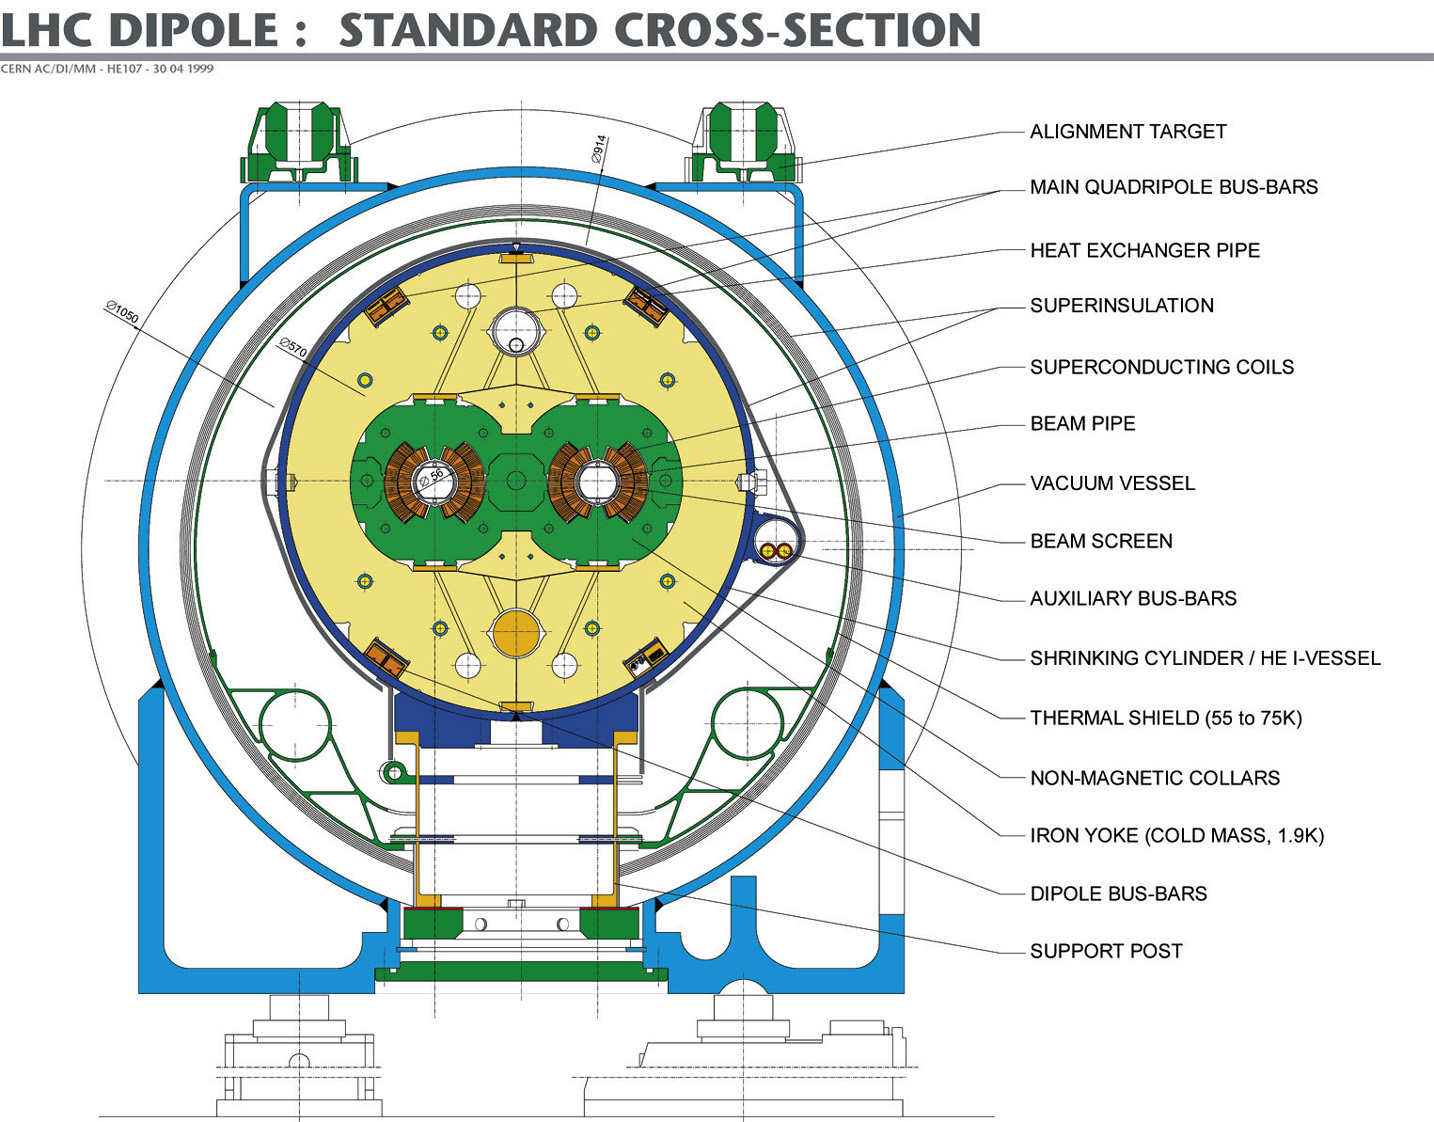
\includegraphics[width=0.75\textwidth]{figures/LHC/LHC_dipole.jpg}
    \caption[]{The cross-section of an LHC dipole magnet with vacuum chamber~\cite{Team:40524}.}
    \label{fig:lhc_dipole}
\end{figure}

Before entering the LHC, the proton beams went through a sequence of accelerators, as shown in Figure~\ref{fig:cern_complex}, which gradually increased the beams' energy. 
A single bottle of Hydrogen gas serves as the sole proton source for the whole LHC. 
At the LINAC2 linear accelerator site, the hydrogen gas is introduced into the duoplasmatron, which ionizes the gas to create a plasma of electrons and hydrogen ions~\cite{Burnet:1359959}. The plasma is then manipulated by strong electrical and magnetic fields, which separate and accelerate the protons out of the duoplasmatron and into the accelerator. 
The protons enter the LINAC2 at about 90 keV and are accelerated to 50 MeV before arriving in the Booster.
The Booster is a (relatively) small synchrotron, followed by the Proton Synchrotron (PS) and Super Proton Synchrotron (SPS). The proton beam is accelerated gradually at each stage and split before entering the LHC as two countercirculating beams. The details of this process are summarized in Table~\ref{table:accelerators}.

Within the synchrotrons, the proton beam is repeatedly passed through the radiofrequency (RF) cavities, metallic chambers containing an electromagnetic field.
This process accelerates the protons and organizes them into bunches with 25 ns spacing.
Once the proton bunches circulate in the LHC, they are further accelerated while maintaining a 25 ns spacing. The beams can circulate stably in the LHC for many hours and only need to be refilled if the beam is dumped~\cite{LyndonEvans_2008}.

\begin{figure}[ht]
    \centering
    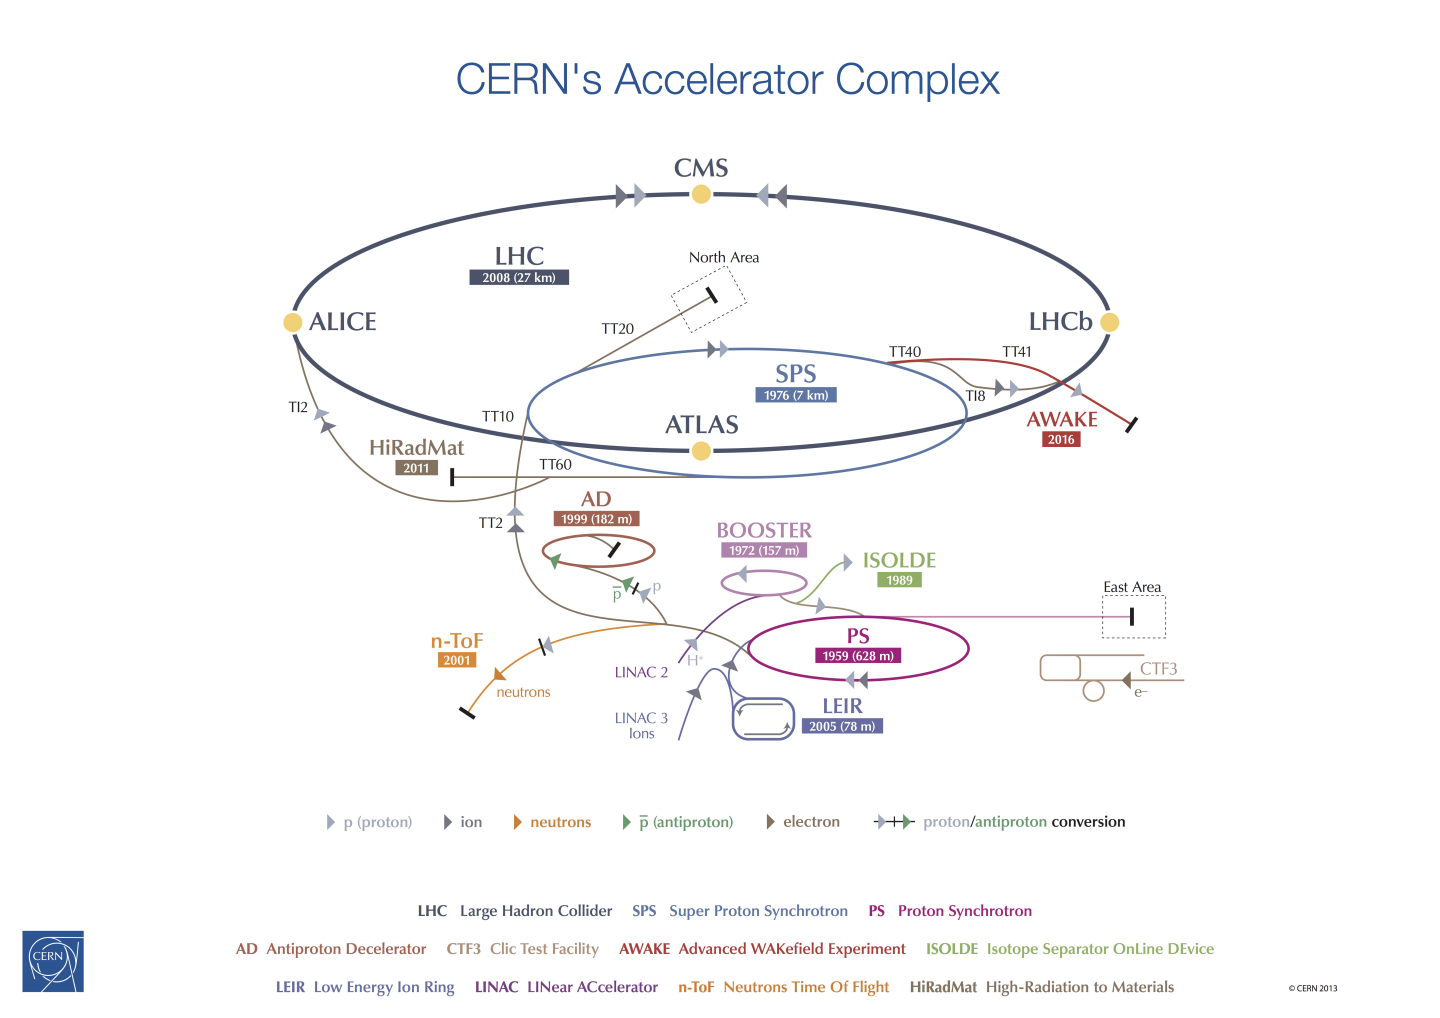
\includegraphics[width=0.8\textwidth]{figures/LHC/CERN_ComplexL.jpg}
    \caption[]{The CERN accelerator complex~\cite{Haffner:1621894}. The LHC proton injector chain is denoted by the light grey arrows.}
    \label{fig:cern_complex}
\end{figure}

\begin{table}[ht]
\centering
\begin{adjustbox}{width=0.95\textwidth}
\begin{tabular}{|l|l|l|l|}
\hline
\textbf{Accelerator Name} & \textbf{Type} & \textbf{Dimensions/Circumference} & \textbf{Exit/Final Energy} \\ \hline
LINAC2 & Linear Accelerator & - & 50 MeV \\ \hline
Booster & Synchrotron & 157 m & 1.4 GeV \\ \hline
Proton Synchrotron (PS) & Synchrotron & 628 m & 26 GeV \\ \hline
Super Proton Synchrotron (SPS) & Synchrotron & 7 km & 450 GeV \\ \hline
Large Hadron Collider (LHC) & Synchrotron & 27 km & 6.5 TeV (per beam) \\ \hline
\end{tabular}
\end{adjustbox}
\caption{Summary of CERN's Accelerator Chain Leading to the LHC}
\label{table:accelerators}
\end{table}

\clearpage
\section{The ATLAS Detector}
The ATLAS (A Toroidal LHC ApparatuS) detector~\cite{TheATLASCollaboration_2008} is a general purpose detector designed to search for all types of interesting physics events at a high luminosity. The ATLAS experiment is one of the four main LHC experiments. The ATLAS detector is located in the experiment cavern at Point 1 of the LHC at the same depth as the tunnel, roughly 100 m underground.

The detector is a large cylindrical shape, 44 m long and 25 m in diameter, and weighs approximately 7000 tonnes. Figure~\ref{fig:atlas_scale} shows the sub-detector systems of ATLAS and the relative human scale. The beam pipe is encased by the Inner Detector (ID), which in turn is surrounded by the calorimeters, and these are all nested inside the muon spectrometer (see Figure \ref{fig:atlas_cross}).
The LHC coordinate system is illustrated as a rectangular coordinate system in Figure~\ref{fig:atlas_coordinate}

\begin{figure}[ht]
    \centering
    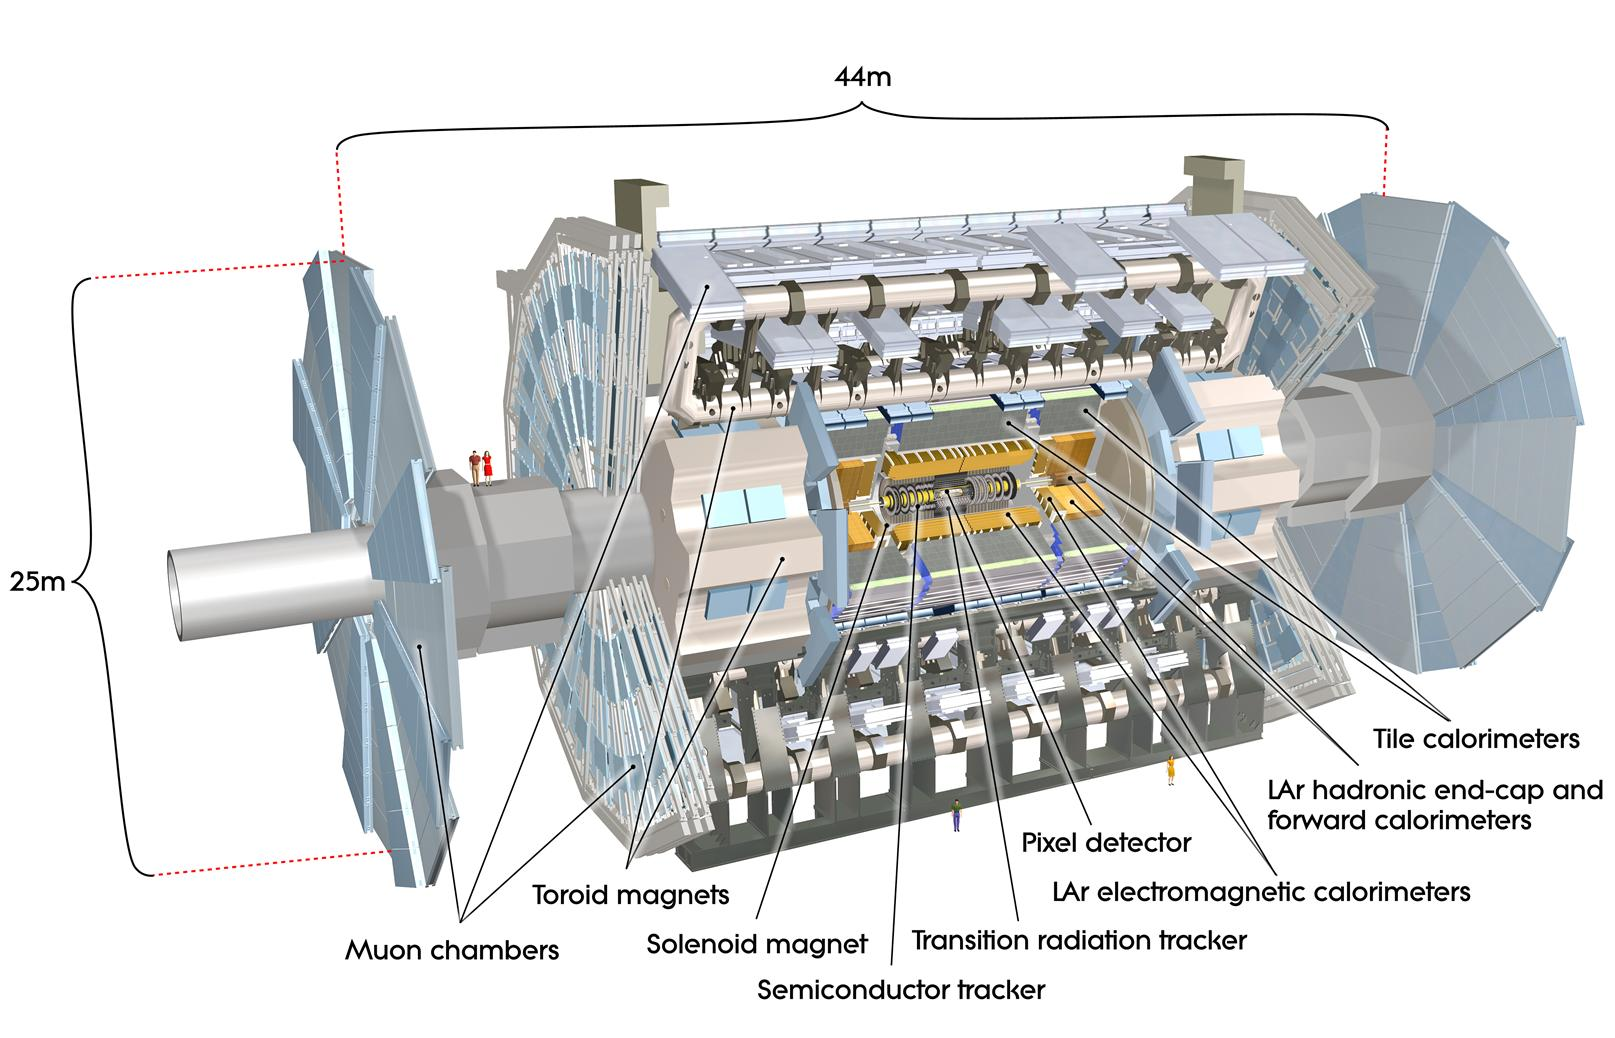
\includegraphics[width=0.85\textwidth]{figures/LHC/atlas_scale.jpg}
    \caption[]{ATLAS detector with human models included for scale~\cite{Pequenao:1095924}.}
    \label{fig:atlas_scale}
\end{figure}

\begin{figure}[ht]
    \centering
    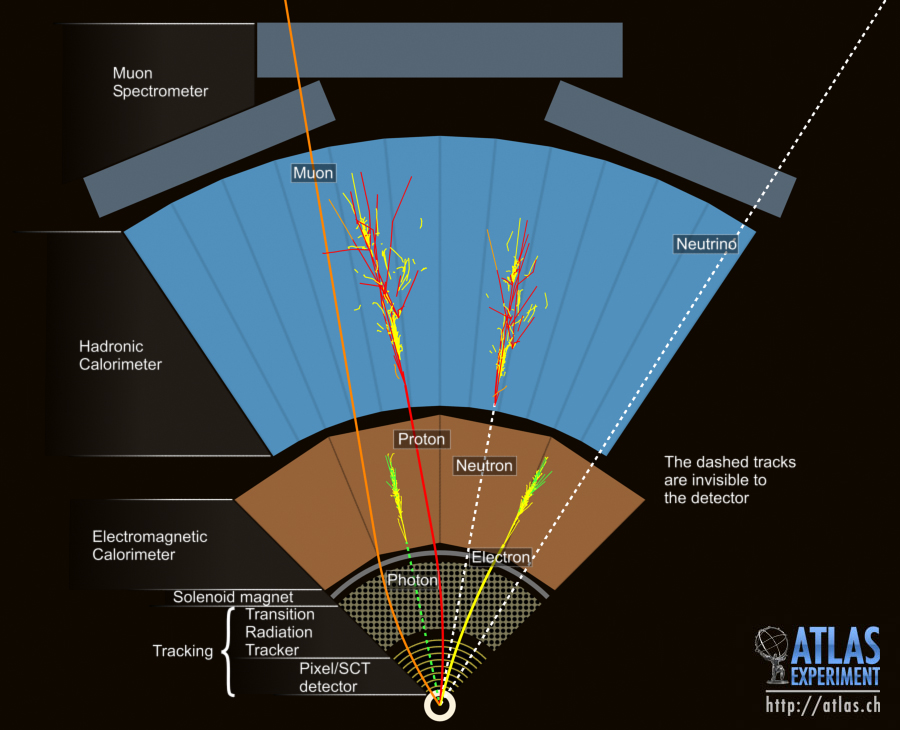
\includegraphics[width=0.75\textwidth]{figures/LHC/atlas_cross.jpg}
    \caption[]{The inner layers of ATLAS, depicted in a cross-sectional view along the x-y plane~\cite{Pequenao:1095924}.}
    \label{fig:atlas_cross}
\end{figure}

\begin{figure}[ht]
\centering
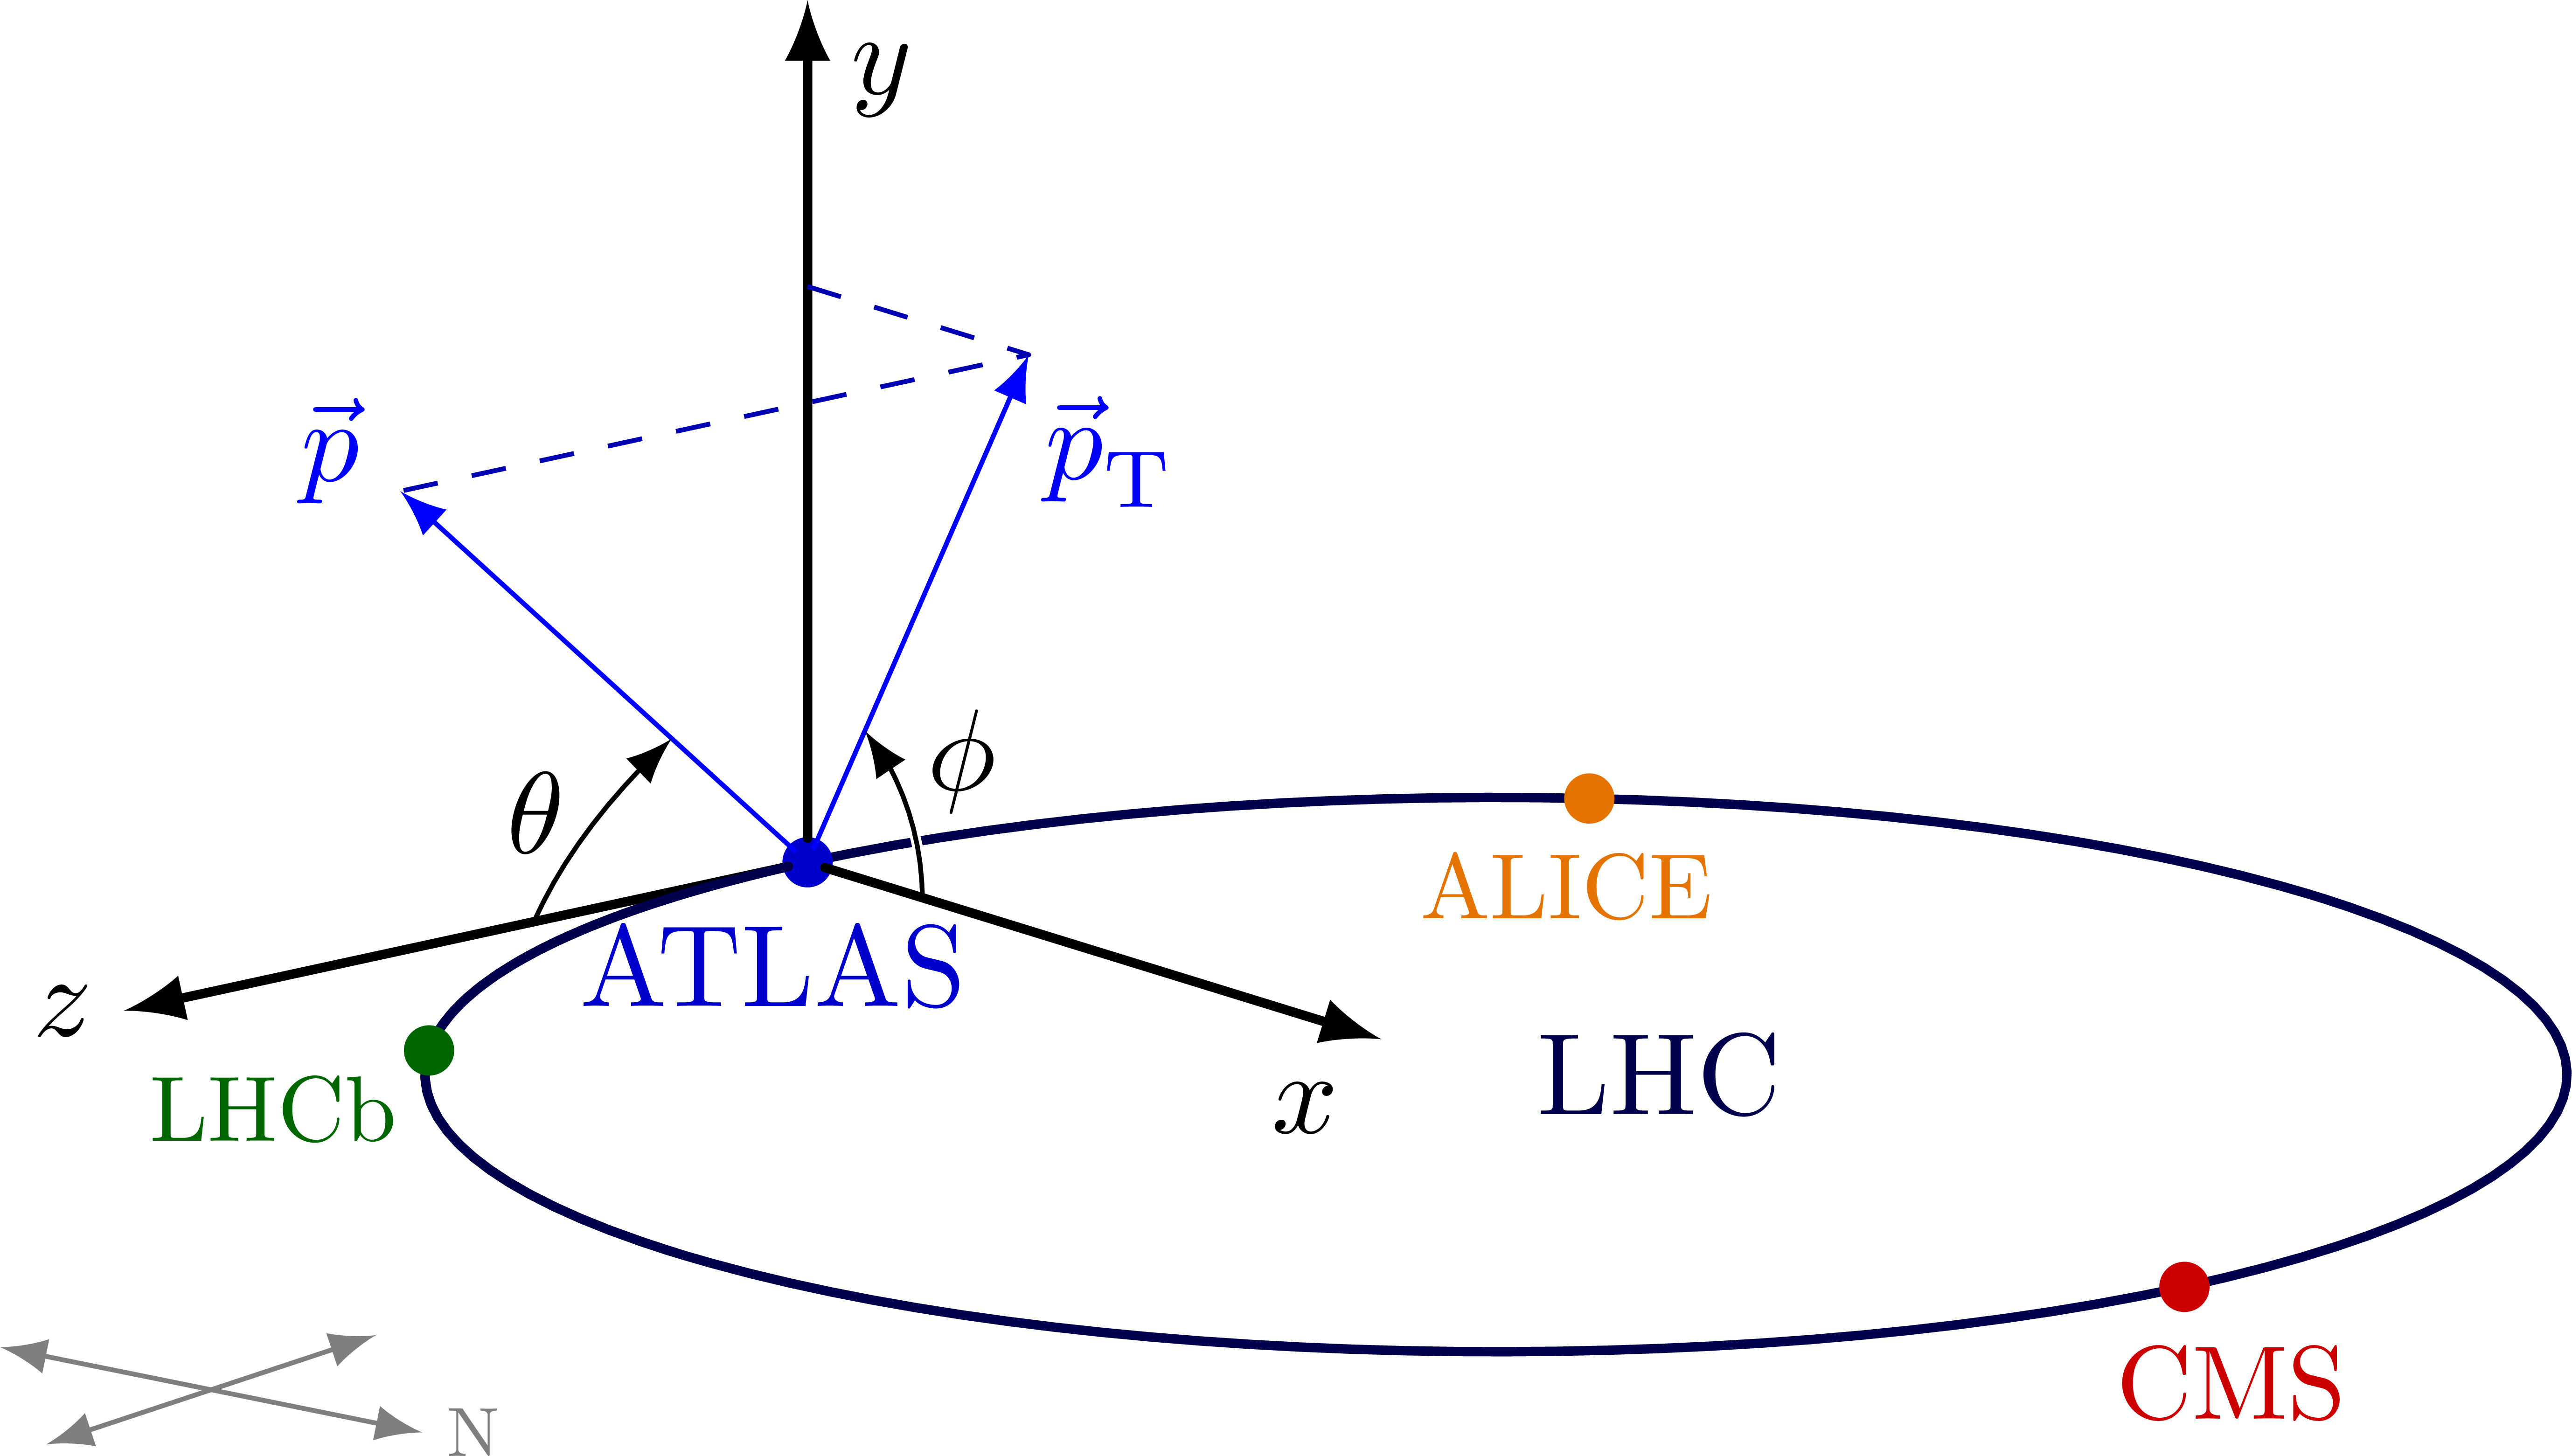
\includegraphics[width=0.75\textwidth]{figures/LHC/axis3D_CMS-003.png}
\caption[The LHC coordinate system]{The LHC coordinate system as seen from the ATLAS detector~\cite{neutelings2023lhc}.}
\label{fig:atlas_coordinate}
\end{figure}

In the transverse plane of this right-handed coordinate system, positive x points toward the center of the LHC ring, and positive y points toward the sky.
The beam pipe defines the orientation of the z-axis, with the positive direction going counterclockwise around the LHC ring.
While the LHC coordinate system is Cartesian, the coordinate system preferred for describing LHC events, particularly in the ATLAS experiment, utilizes a particle's transverse momentum ($p_T$), pseudorapidity ($\eta$), and azimuthal angle ($\phi$). The polar angle ($\theta$) is defined relative to the beam axis, whereas the azimuthal angle ($\phi$) is measured in the plane perpendicular to the beam.
In practice, pseudorapidity is preferred over the polar angle. It is defined as
\begin{equation}
    \eta = -\ln \left( \tan \frac{\theta}{2} \right)
\end{equation}
and is a good approximation of the rapidity of a particle in the high-energy regime, which is a measurement of the particle's velocity along the beam axis, given by
\begin{equation}
    y = \frac{1}{2} \ln \left( \frac{E + p_z}{E - p_z} \right).
\end{equation}

While neither the rapidity nor the pseudorapidity are Lorentz invariants, the rapidity difference between the two particles is invariant under Lorentz boosts along the direction of motion. Similarly, the difference in pseudorapidities is approximately invariant under such boosts, especially for highly relativistic particles in LHC/ATLAS events.

%%%ID
\subsection{The Inner Detector}
Located inside the solenoid magnet, the Inner Detector (ID)~\cite{ATLAS:1998yql} consists of three subsystems designed to detect charged particles, covering a pseudorapidity range of \(|\eta| < 2.5\). As seen in Figure~\ref{fig:id_layout}, these subsystems are described from the innermost to the outermost as follows.

\begin{figure}[ht]
    \centering
    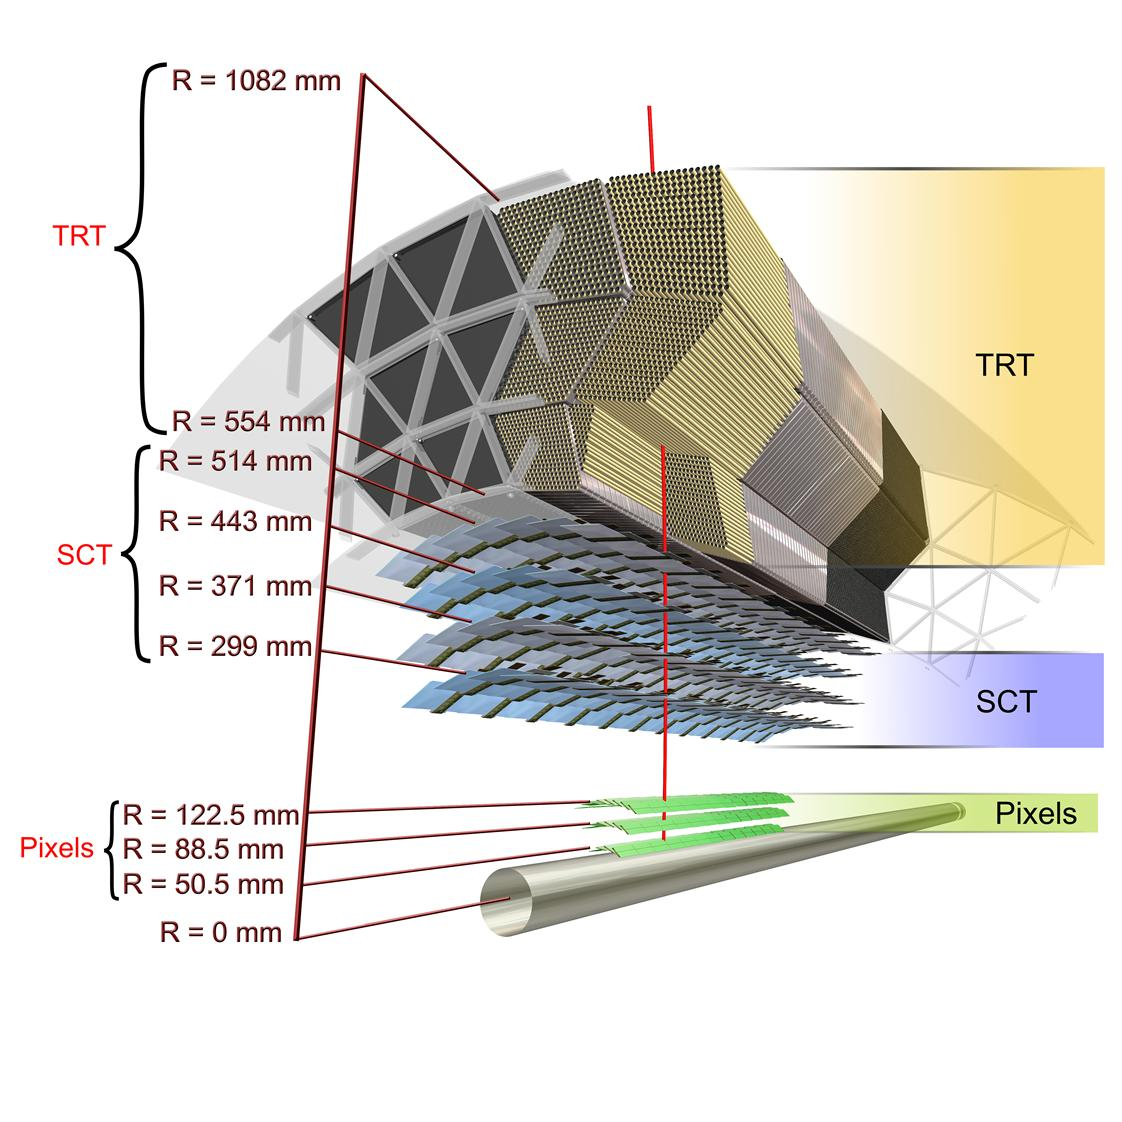
\includegraphics[width=0.75\textwidth]{figures/LHC/id_layout.jpg}
    \caption[]{ATLAS Inner Detector cut-away: Pixel Detector, Semiconductor Tracker, and Transition Radiation Tracker~\cite{Pequenao:1095926}.}
    \label{fig:id_layout}
\end{figure}

The first, the Pixel detector, consists of four layers of pixel detectors.
These pixel layers comprise a two-dimensional array of silicon pixels, providing high-precision measurements close to the interaction point.
The innermost layer is the Insertable B-Layer (IBL). The ``B'' in its name stands for ``Barrel,'' though the IBL is crucial in detecting short-lived particles, like hadrons with $b$ quarks. Due to its closeness to the interaction point, the IBL enhances the performance of the Pixel detector by improving the precisions of vertexing and track reconstruction.

The second subsystem, the SemiConductor Tracker (SCT), comprises four double layers of silicon strips. The SCT behaves similarly to the Pixel detector, except the measurement is one-dimensional. 
When a charged particle moves through a silicon layer, it bumps electrons to a higher energy level, creating ``holes'' in their place. This generates a current and signal the detector can read as a ``hit.''

The last subsystem is the Transition Radiation Tracker (TRT)~\cite{TheATLASTRTcollaboration_2008}, a straw tracker comprised of approximately 300,000 4 mm-diameter straw tubes. 
A straw tube is a long tube with a wire in the center filled with gas (Xenon). When a charged particle passes through, the gas becomes ionized, creating an electronic signal (a ``hit'').
The superconducting solenoid magnet bends the paths of charged particles based on their momentum, with the numerous hits in the TRT greatly enhancing momentum measurement accuracy.

\subsection{The Calorimeters}
The calorimeter system, enclosing the solenoid magnet and the inner detector, provides coverage up to \(|\eta| < 4.9\), although the coverage varies for each subdetector.
The calorimeters employs a fundamentally different detection method compared to the ID. While the ID is designed to track particles with minimal interaction, the calorimeters are designed to completely absorb the particles. This absorption prevents most particles from reaching further layers of detection. A significant advantage of calorimeters is their ability to detect neutral particles, with the exception of neutrinos. The calorimeter system comprises various subsystems, each responsible for covering a specific range of particles. Figure~\ref{fig:cal_layout} illustrates these subsystems.

\begin{figure}[ht]
    \centering
    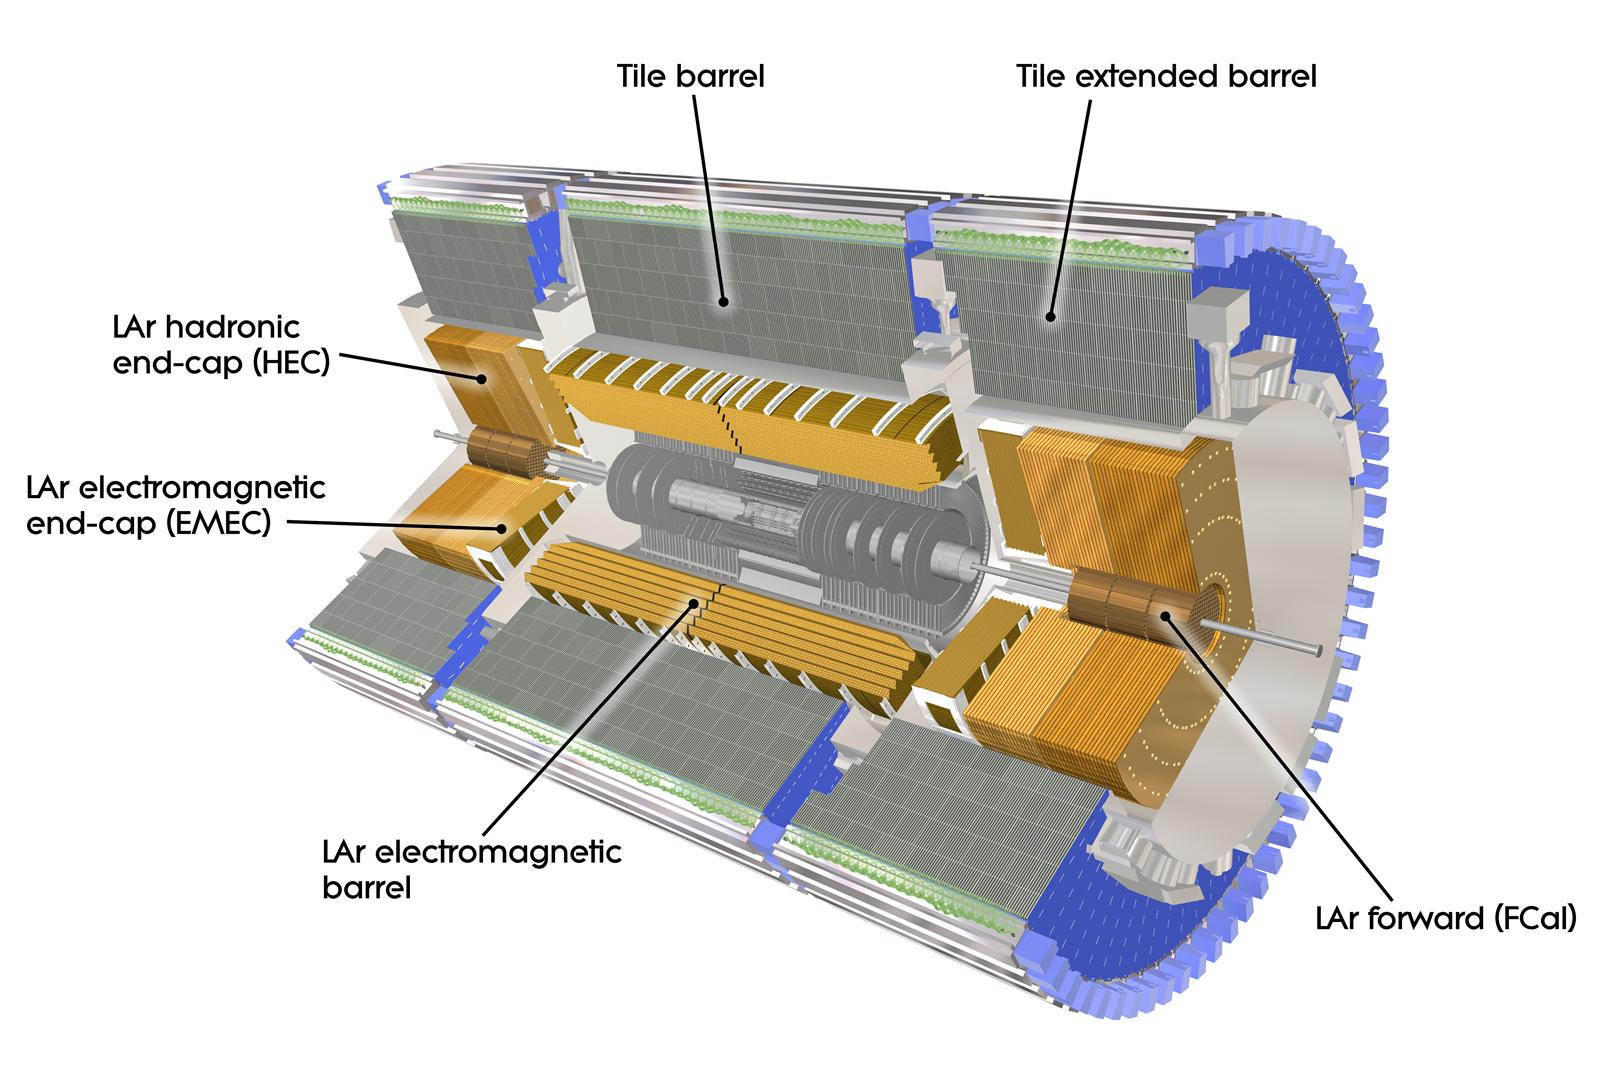
\includegraphics[width=0.75\textwidth]{figures/LHC/cal_layout.jpg}
    \caption[]{Cut-away view of the ATLAS calorimeter system~\cite{Pequenao:1095927}.}
    \label{fig:cal_layout}
\end{figure}

Calorimeters operate on a fundamental principle where particles enter a region filled with dense matter, leading to the creation of particle showers as they release their energy within the calorimeter. These devices are typically constructed from alternating layers of materials: a dense material that absorbs the particles, and a sampling material positioned between the absorber layers. The purpose of the sampling material is to detect the particle showers generated by the absorbers.
This detection is achieved through sensors connected to the sampling material. There are two prevalent types of sampling materials used in calorimeters: scintillating plastics and ionizable liquids. Scintillating plastics emit light when struck by particles and are read by photodiodes, while the ionizable liquids create ions that are detected by electrodes.

The innermost section of the calorimeter is occupied by the Electro-Magnetic Calorimeter (ECAL)~\cite{ATLAS:1996ab}. Noted for its unique accordion design, the ECAL ensures complete azimuthal coverage, eliminating gaps along the azimuthal direction. Despite this, a gap exists between the barrel and endcap sections of the ECAL along the $z$-direction, leading to a common practice of excluding particles within the pseudorapidity range of \(1.37 < |\eta| < 1.52\). The ECAL employs lead as the primary absorbing material, complemented by steel, and utilizes liquid argon as the sampling medium. Upon interaction with incoming particles, the liquid argon becomes ionized. These ionization events are then detected by electrodes shaped to match the accordion design of the calorimeter. The coverage of the ECAL extends to a pseudorapidity range of \(|\eta| < 3.2\).

The principal hadronic calorimeter, known as TileCAL~\cite{ATLAS:1996aa}, is designed to accommodate the penetrating nature of hadrons, which travel deeper into materials before stopping. TileCAL is considerably larger, utilizing steel as its absorbing material and scintillating plastic as the sampling material, ensuring effective energy measurement of hadrons. TileCAL is specifically engineered to cover a pseudorapidity range of \(|\eta| < 1.7\). In contrast, the endcaps of the calorimeter, which are constructed differently, employ copper as the absorbing material and liquid argon as the sampling medium. These endcaps extend the calorimeter's coverage to a range of \(1.5 < |\eta| < 3.2\), complementing TileCAL. Due to the endcaps being nested within TileCAL's structure, there is a significant degree of overlap between these components, ensuring that there are no gaps in the hadronic calorimeter's coverage.

The Forward Calorimeter (FCAL)~\cite{AArtamonov_2008} plays a crucial role in capturing particles that travel almost parallel to the beam line, essential for accurately measuring missing energy in experiments. Its design enables it to cover an extended pseudorapidity range of \(3.1 < |\eta| < 4.9\), significantly beyond the coverage of the central detectors. Although most physics analyses focus on events within a much narrower range, the ability of the FCAL to detect particles in this extended range is vital for ensuring that no energy goes unaccounted for, which is crucial for precision measurements. The FCAL comprises two distinct sections: an inner section with copper as the absorbing material and an outer section that utilizes tungsten. Liquid argon is employed as the sampling material across the entire FCAL, facilitating the detection and measurement of particle energies.


\subsection{The Muon Spectrometer}

The muon spectrometer (MS)~\cite{ATLAS:1997ad}, designed to detect muons within \(|\eta| < 2.7\), encircles the calorimeters and forms the detector's outermost layer. Its barrel region is defined in the range of \(|\eta| < 1.05\), with the endcap regions covering the remaining area.
The MS is supplemented by three large toroid magnets surrounding the calorimeters, bending the charged particles in the z direction with a strength of about \(2.5 \, \text{T}\cdot\text{m}\) in the barrel region and up to \(6 \, \text{T}\cdot\text{m}\) in the endcaps.
Only muons and neutrinos, due to their unique properties, can penetrate the calorimeters to reach the MS, which is specifically designed for precise measurements of muon momentum.
As seen in Figure~\ref{fig:muon_spec}, the trigger system of the muon system features the Resistive Plate Chamber (RPC) and Thin Gap Chamber (TGC). These trigger chambers offer bunch-crossing identification, well-defined transverse momentum (\pt) thresholds, and measurements of the muon's track coordinate~\cite{TheATLASCollaboration_2008}.
Combined with the corresponding measurements from the ID, one can determine all three components of a muon's momentum.

\begin{figure}[ht]
    \centering
    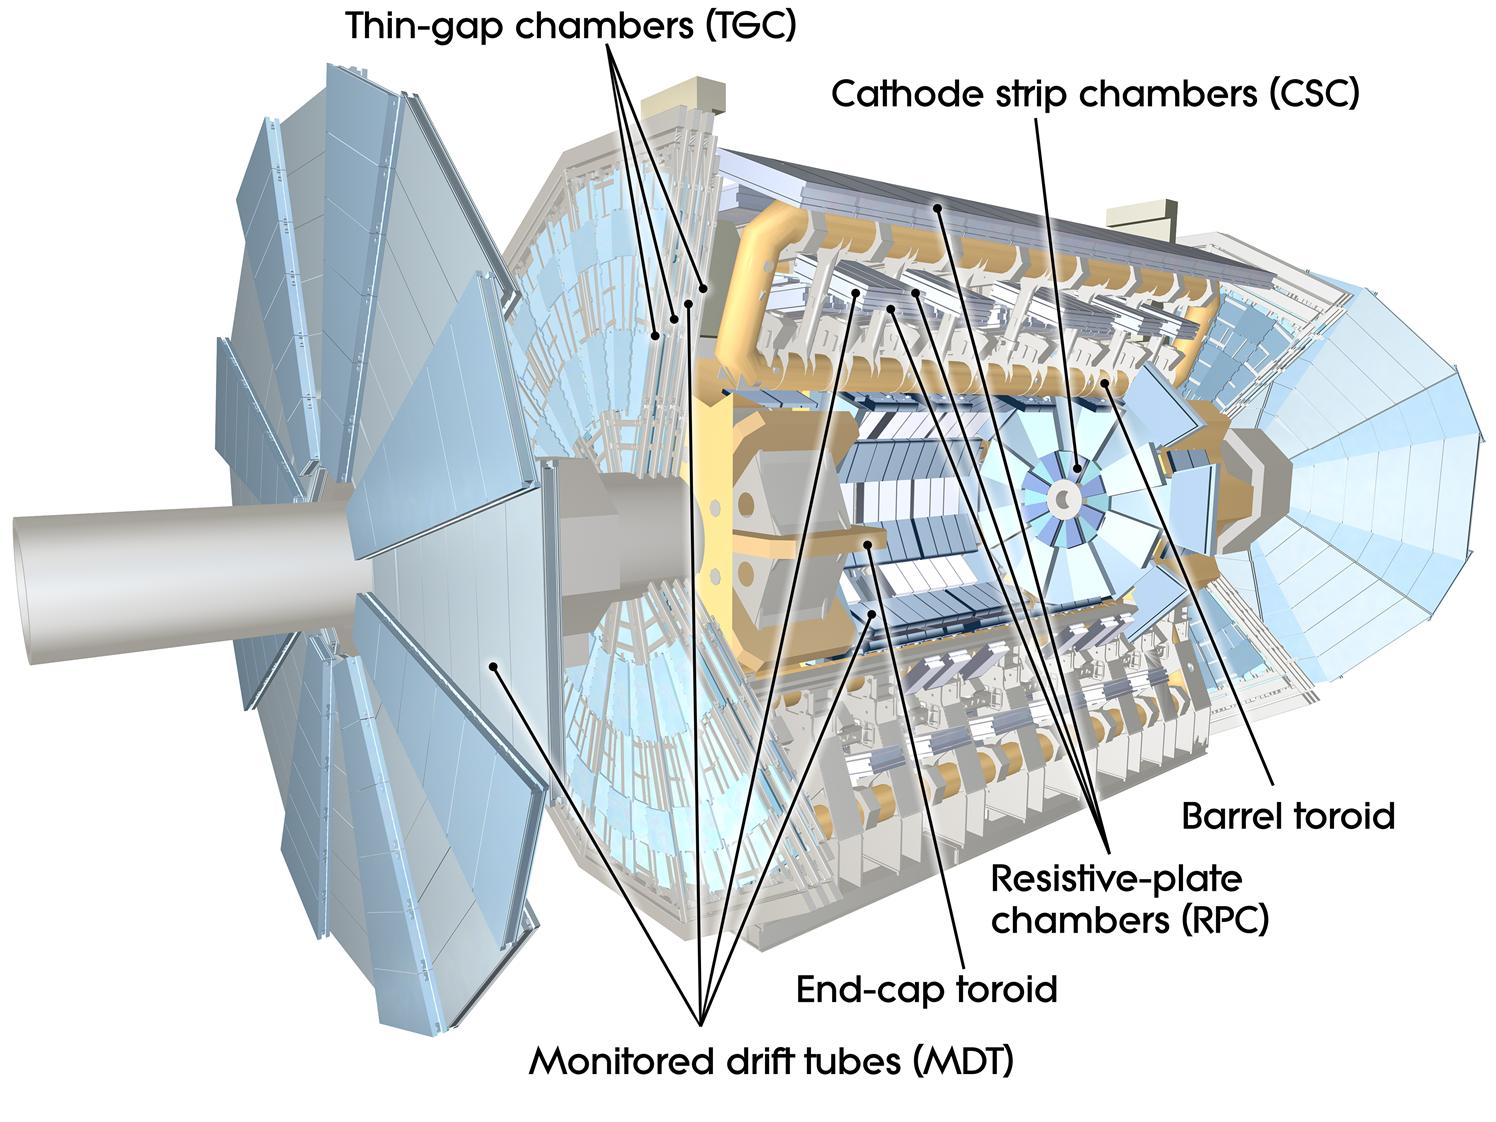
\includegraphics[width=0.75\textwidth]{figures/LHC/muon_spec.jpg}
    \caption[]{Cut-away view of the Muon Spectrometer system~\cite{Pequenao:1095929}.}
    \label{fig:muon_spec}
\end{figure}

%Pequenao:1095929


%TDAQ
\clearpage
\section{The Trigger and Data Acquisition}
\label{The_Trigger_and_Data_Acquisition}
The Trigger and Data Acquisition (TDAQ) system of ATLAS decides which events to record and store. As mentioned in Section~\ref{the_lhc}, the 25 ns spacing between proton bunches results in an event rate of 1 GHz, making real-time storage unfeasible.
Since the vast majority of the events aren't interesting for physics analysis here at ATLAS, TDAQ's goal is to reduce the collection rate to 1.5 kHz.
The trigger system is comprised of two triggers: the hardware-based Level 1 Trigger (L1)~\cite{ATLAS:1998ad} and the software-based High Level Trigger (HLT)~\cite{ATLAS:2003aa}.
Figure~\ref{fig:tdaq_layout} illustrates how the system works.

\begin{figure}[ht]
    \centering
    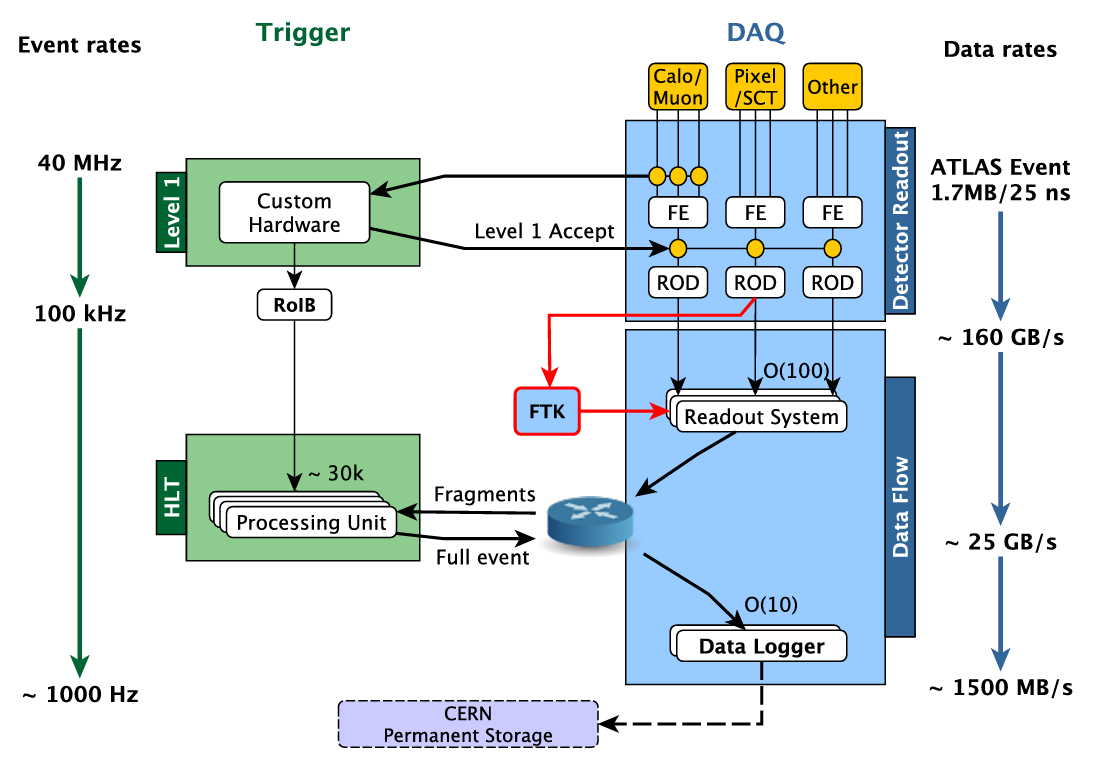
\includegraphics[width=0.85\textwidth]{figures/LHC/tdaq_1.png}
    \caption[]{ATLAS TDAQ Architecture~\cite{Abbott_2016}.}
    \label{fig:tdaq_layout}
\end{figure}

The L1 trigger, directly connected to the muon spectrometer and the calorimeters, identifies physics events with interesting objects such as high-momentum muons, significant missing energy, high-energy electrons/photons, or high-energy hadrons.
The dedicated hardware for the L1 trigger is situated within the same cavern as the ATLAS detector.
Events passing the L1 trigger are transferred from the detectors' Front End (FE) to the Read Out Drivers (ROD) at a reduced the event rate of 100 kHz.

The HLT includes the Level 2 Trigger (L2) and the Event Filter (EF). L1 identifies a region of interest (ROI) of the detector, and the complete event data within this ROI is forwarded to L2. 
``Tracking'' in the ROI is done by L2 to reconstruct the trajectory (or track) of electrically charged particles in the ID.
The tracks and calorimeter information are combined to refine the object selection with higher resolution than what was used in L1, such as tighter requirements on electrons, muons, and missing energy.
Events that pass L2 requirements are sent to the EF, which uses data from the entire detector to decide whether to keep the event.



%%%FTK
\section{Fast Tracker}

The Fast TracKer (FTK) system was foreseen as a significant upgrade for the TDAQ system of ATLAS by providing hardware-based tracking information directly to the HLT.
As discussed in Section 3.3, although the L1 trigger and HLT perform exceptionally in selecting physics events and reducing the event rate, this implementation does have its limitations.
Currently, the HLT receives the "hits" information recorded by the ID, essentially points in space, and conducts tracking calculations within the ROIs determined by the L1 trigger.
Tracking calculations in the HLT software are demanding and slow, leading to restrictions on the size and number of ROIs. 
The ROI approach also resulted in notable inefficiencies in jet finding, due to discrepancies between the online and offline strategies~\cite{TAMSETT2013253}~\cite{Aad2016}.
A solution is to use specialized hardware for this task, which is the primary goal of the FTK system. FTK will be positioned between the L1 trigger and HLT, offering tracking information for all events that pass the L1 trigger across the entire detector and supplying this data to the HLT.

The FTK system consists of various types of boards and components, with details provided in Figure~\ref{fig:ftk_overview} and Table~\ref{table:ftk_overview}. The Input Mezzanines (IM) receive data directly from the Level 1 trigger (the RODs). There are a total of 12 layers from the Inner Detector: four double SCT layers, three Pixel layers, and one IBL.
Clustering is applied to the hits from these layers to reduce data flow. The clustered data is then sent to the Data Formatter (DF) system.
The DF system divides the data, sending eight layers (five from the SCT and three from the Pixel) to the main Processing Units (PU) and the remaining four layers (three SCT and one IBL) to the Second Stage Boards (SSB).

\begin{figure}[ht]
  \centering
  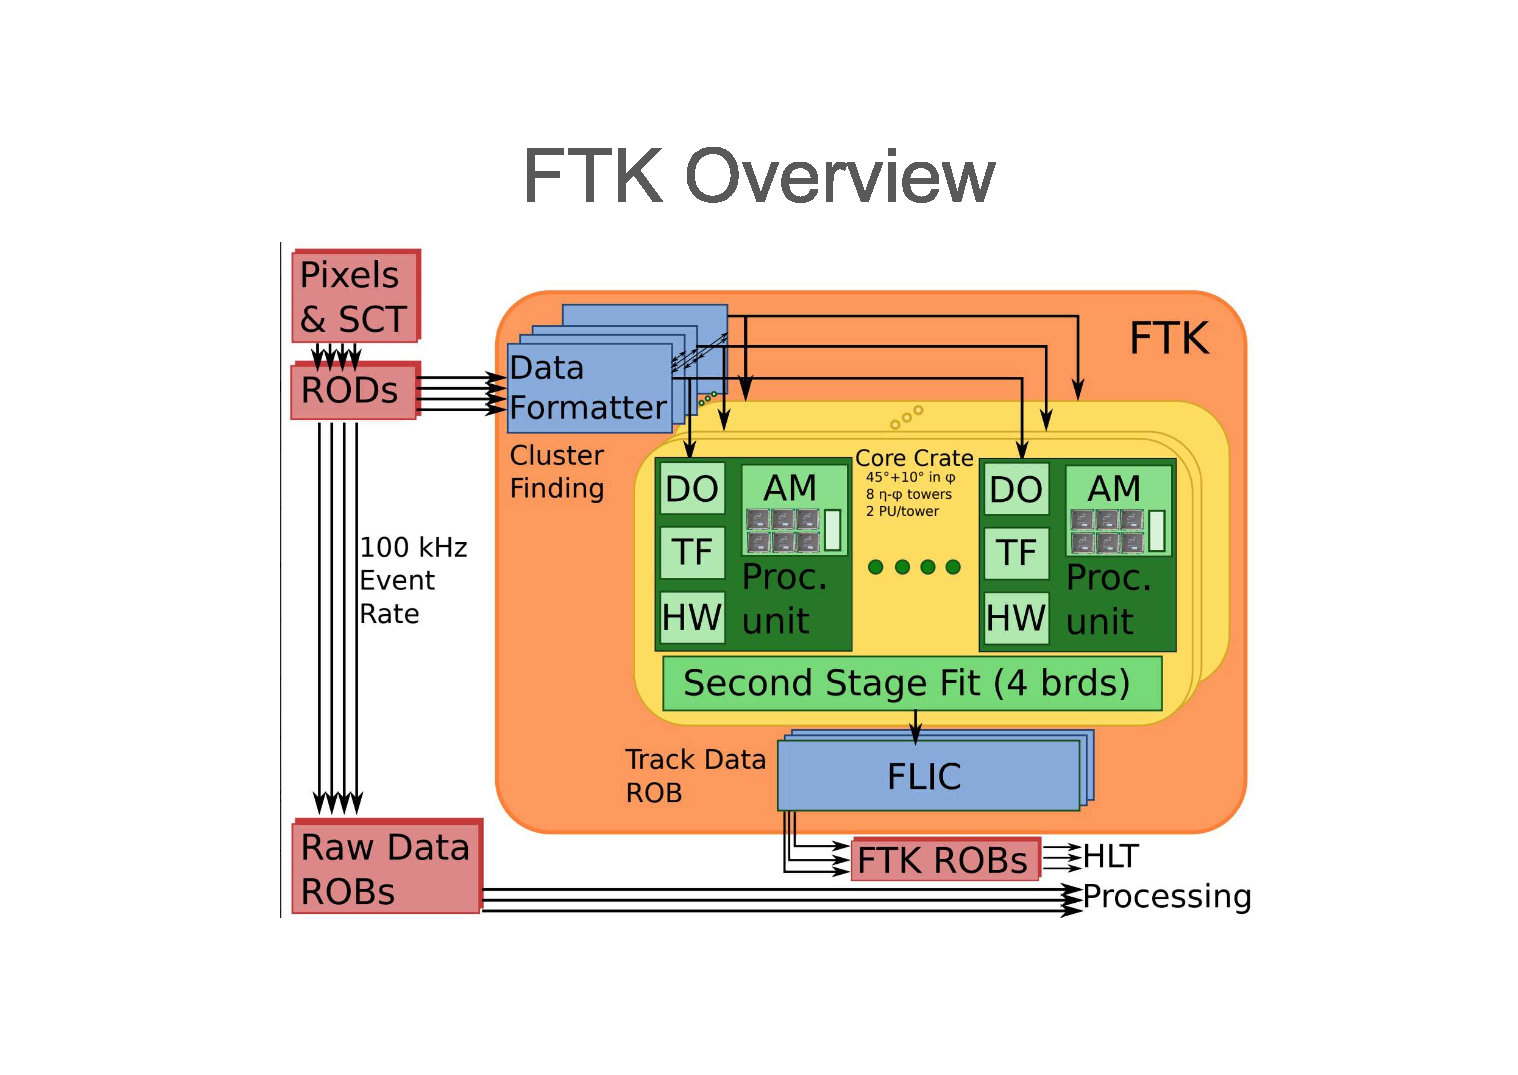
\includegraphics[width=0.95\textwidth]{figures/ftk/ftk_overview.pdf}
  \caption{Overview of the FTK system.}
  \label{fig:ftk_overview}
\end{figure}

\begin{table}[ht]
\centering
\resizebox{0.95\textwidth}{!}{%
\begin{tabular}{llllr}
\hline
\textbf{Module} & \textbf{Function} & \textbf{Type} & \textbf{Number} \\
\hline
\hline
IM & Input Mezzanine & Cluster Pixel and SCT hits, format module data & Mezzanine & 128 \\\hline
DF & Data Formatter & Transport and duplicate module hit data to \(\eta\)-\(\phi\) towers & ATCA & 32 \\\hline
AUX & Auxiliary Card & Transport coarse-resolution 8-layer hit data to AMB & VME & 128 \\\hline
AMB & AM Board & Transport hit data to AM & VME & 128 \\
AM & Associative Memory & Match hits to patterns & ASIC & 8192 \\
AUX & Auxiliary Card & Evaluate track candidates in matched patterns & VME & 128 \\\hline
SSB & Second Stage Board & Add remaining hits to 8-layer tracks, fit, remove overlaps & VME & 32 \\\hline
FLIC & HLT Interface Board & Interface to ATLAS readout & ATCA & 2 \\
\hline
\end{tabular}%
}
\caption{Overview of the FTK system in the order in which the data are processed. 
The AUX appears in the table twice because of its dual functions \cite{Aad_2021}.}
\label{table:ftk_overview}
\end{table}

The main Processing Units are made up of two boards: the Associated Memory Board (AMB) and the Auxiliary Board (AUX), with the AUX serving as a rear transmission module. The AMB is essential to the FTK system. To construct tracks rapidly, billions of precomputed tracks are stored in a large memory bank. These track patterns are then matched to the incoming hit coordinates using massive parallel processing. Each AMB can match eight million patterns in parallel to the incoming hit data.

The Auxiliary Board (AUX) communicates with its corresponding Associated Memory Board (AMB) via the VME backplane, performing a range of functions. Its principal duty involves eight-layer track fitting. The procedure is as follows:
\begin{itemize}
    \item Input data from the DF is forwarded to the AMB.
    \item The AMB, after matching patterns, returns them to the AUX.
    \item Utilizing these patterns, the AUX conducts a fit to assess their quality, allowing tracks to be missing a hit on one layer -- these are termed \textit{majority tracks} -- to boost efficiency.
    \item Moreover, the AUX undertakes the removal of duplicates among the eight-layer track candidates.
    \item Valid eight-layer tracks are then forwarded to the Second Stage Boards (SSB).
\end{itemize}

The Second Stage Board (SSB) system includes 32 boards, each responsible for managing tracks from four PUs. The SSB integrates these eight-layer tracks with hit data for the four additional layers from the corresponding DF, to assemble 12-layer tracks. This process involves:
\begin{itemize}
    \item Extrapolating the eight-layer track into the missing layers.
    \item Using hits near the extrapolated coordinates to fit full 12-layer tracks.
\end{itemize}
Like in the first stage, it is possible for tracks to be missing a hit in one of the new layers. After fitting, tracks undergo a global duplicate check before being forwarded to the FTK Level2 Interface Crate (FLIC). SSBs are paired to cover the entire detector range, with pairs linked in a ring to manage overlap.

The FTK Level2 Interface Crate (FLIC) is the last element in the FTK system, serving two primary purposes:
\begin{itemize}
    \item It merges the 12-layer track data from the 32 SSBs.
    \item It formats the consolidated data so that it can be interpreted by the Read Out System (ROS).
\end{itemize}

\subsection{Second Stage Board}

The Second Stage Boards (SSBs), designed and manufactured at the University of Illinois, perform three critical functions (see Figure~\ref{fig:ssb_board}):
\begin{itemize}
    \item Extrapolating incoming eight-layer tracks to include the missing layers,
    \item Fitting these extrapolations to form 12-layer tracks,
    \item Removing any duplicates found across the detector.
\end{itemize}
The hardware of the SSBs includes five Field-Programmable Gate Arrays (FPGAs) that require firmware. Four of these FPGAs, designated as the EXTF FPGAs, are dedicated to the tasks of extrapolation and track fitting. The fifth FPGA, known as the Hit Warrior (HW) FPGA, is tasked with duplicate removal. Furthermore, the SSBs are equipped with a substantial amount of Reduced Latency Dynamic Random-Access Memory (RLDRAM) for storing the constants necessary for extrapolation and track fitting calculations.
The layout and the dataflow through the SSB are shown in Figure~\ref{fig:ssb_diagram}.

\begin{figure}[ht]
  \centering
  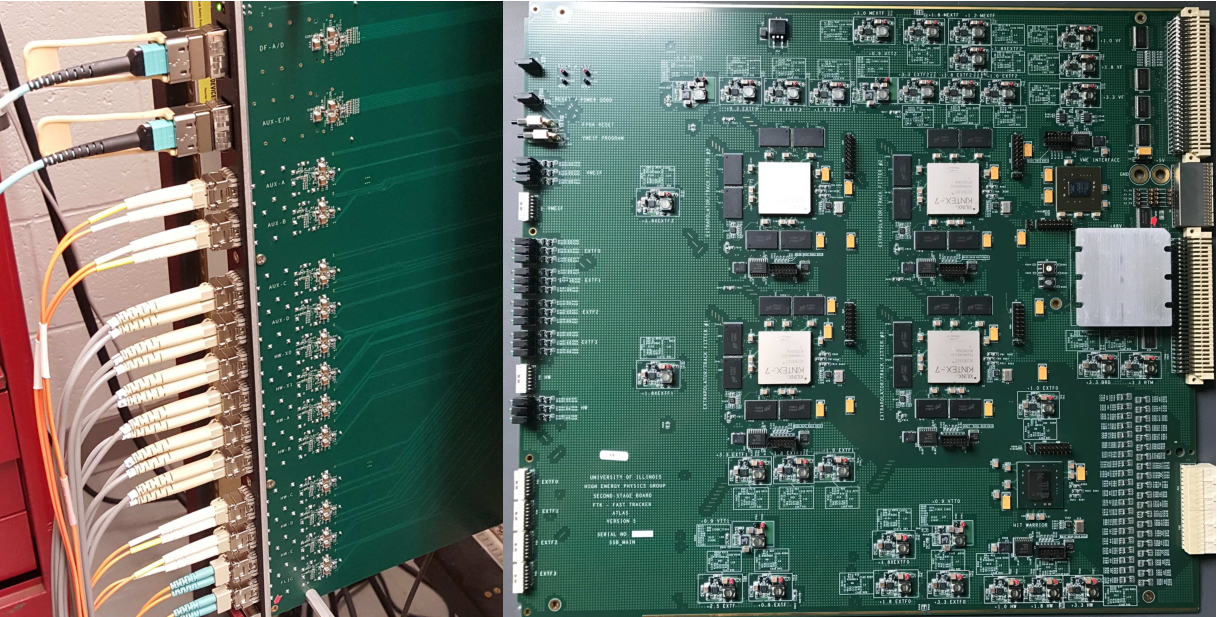
\includegraphics[width=0.75\textwidth]{figures/ftk/ssb_board.pdf}
  \caption{The physical Second Stage Boards~\cite{Aad_2021}.}
  \label{fig:ssb_board}
\end{figure}

\begin{figure}[ht]
  \centering
  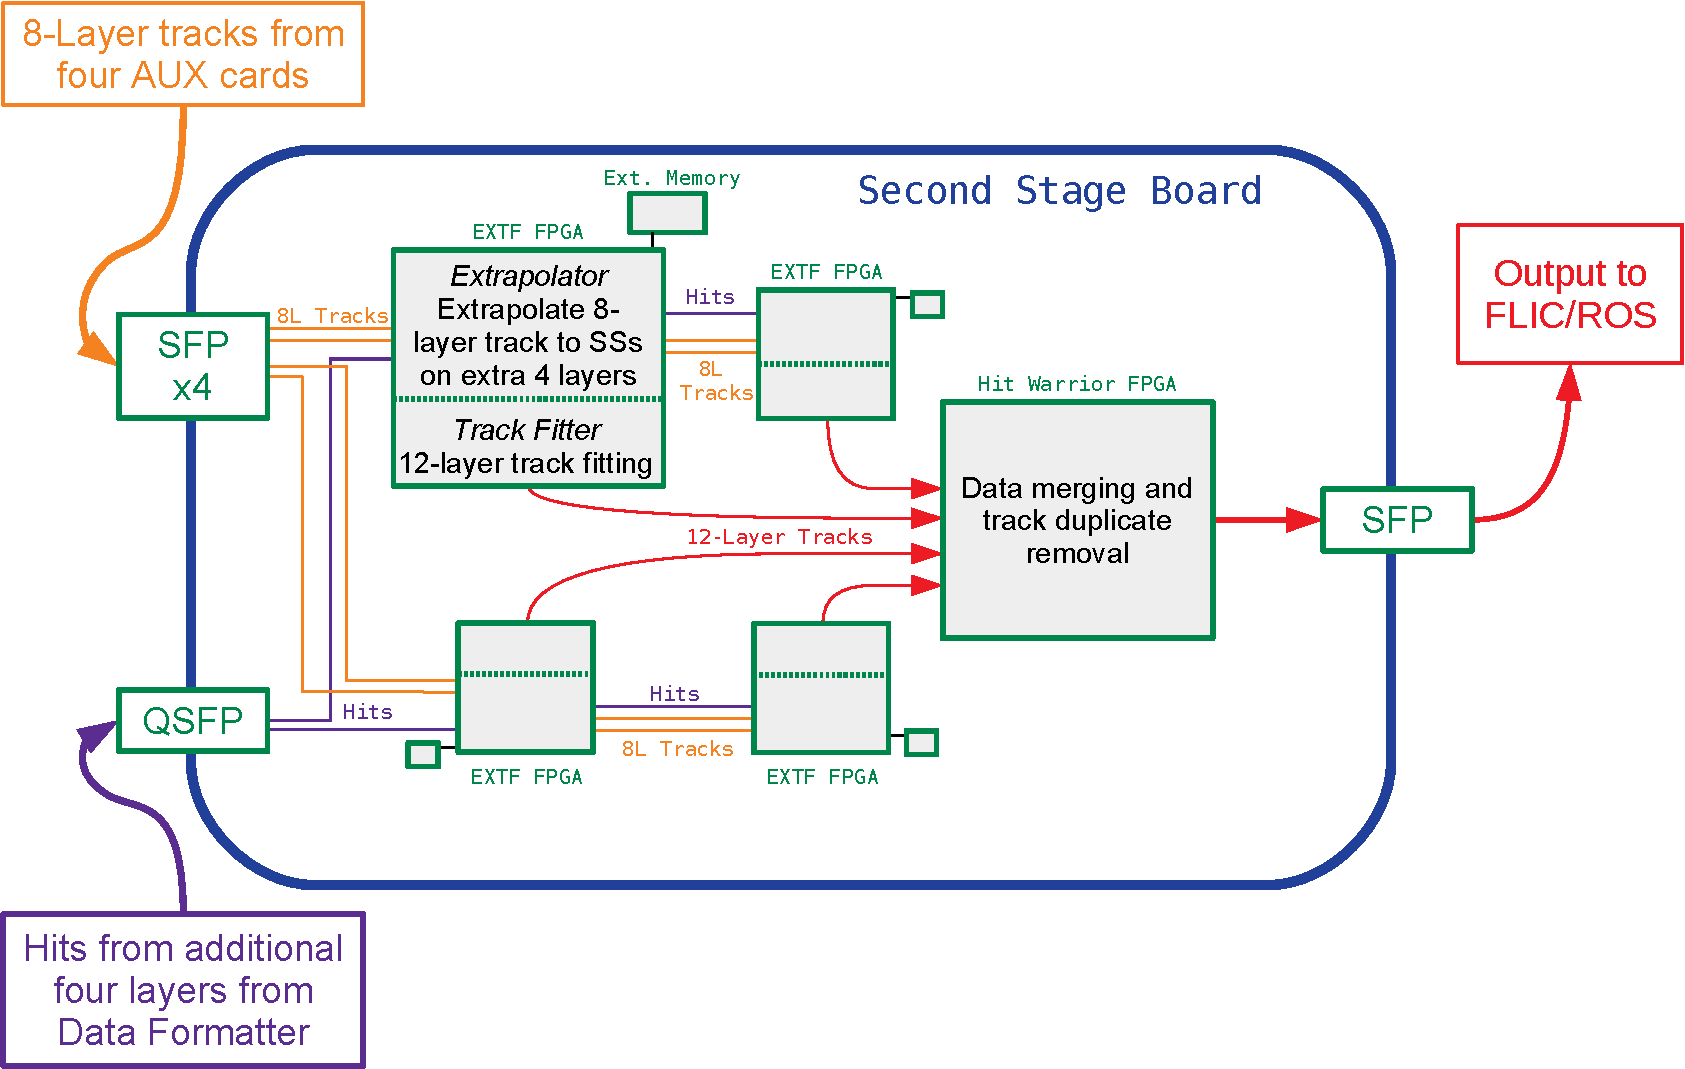
\includegraphics[width=0.75\textwidth]{figures/ftk/ssb_diagram.pdf}
  \caption{Diagram of the dataflow through the Second Stage Board~\cite{Aad_2021}.}
  \label{fig:ssb_diagram}
\end{figure}

The core functionality of the EXTF FPGA is allocated to the Extrapolator (EXP), which oversees the extrapolation process, and the Track Fitter (TF), focused on the fitting of the resulting 12-layer tracks. For a thorough exploration of these firmware aspects, see Markus Atkinson's PhD thesis \cite{Atkinson2019}.

\subsection{Hit Warrior FPGA}
The Hit Warrior FPGA on the SSB serves two key roles. Its main job is to eliminate duplicate tracks. Its second role involves merging data. Each SSB houses four EXTF FPGAs, and the Hit Warrior FPGA collects all their output. This output is then scanned for any duplicates, combined into a single large output packet, and forwarded to the FLIC.
The top-level diagram of the Hit Warrior firmware design is depicted in Figure~\ref{fig:hw_top_diagram}. In the diagram, the Sync Engine module synchronizes the four incoming EXTF streams. The Hit Warrior module is the logic component that performs the comparison and duplicate removal tasks. Additionally, Spy Buffers are utilized for monitoring purposes. More details on the Hit Warrior module follow.

\begin{figure}[ht]
  \centering
  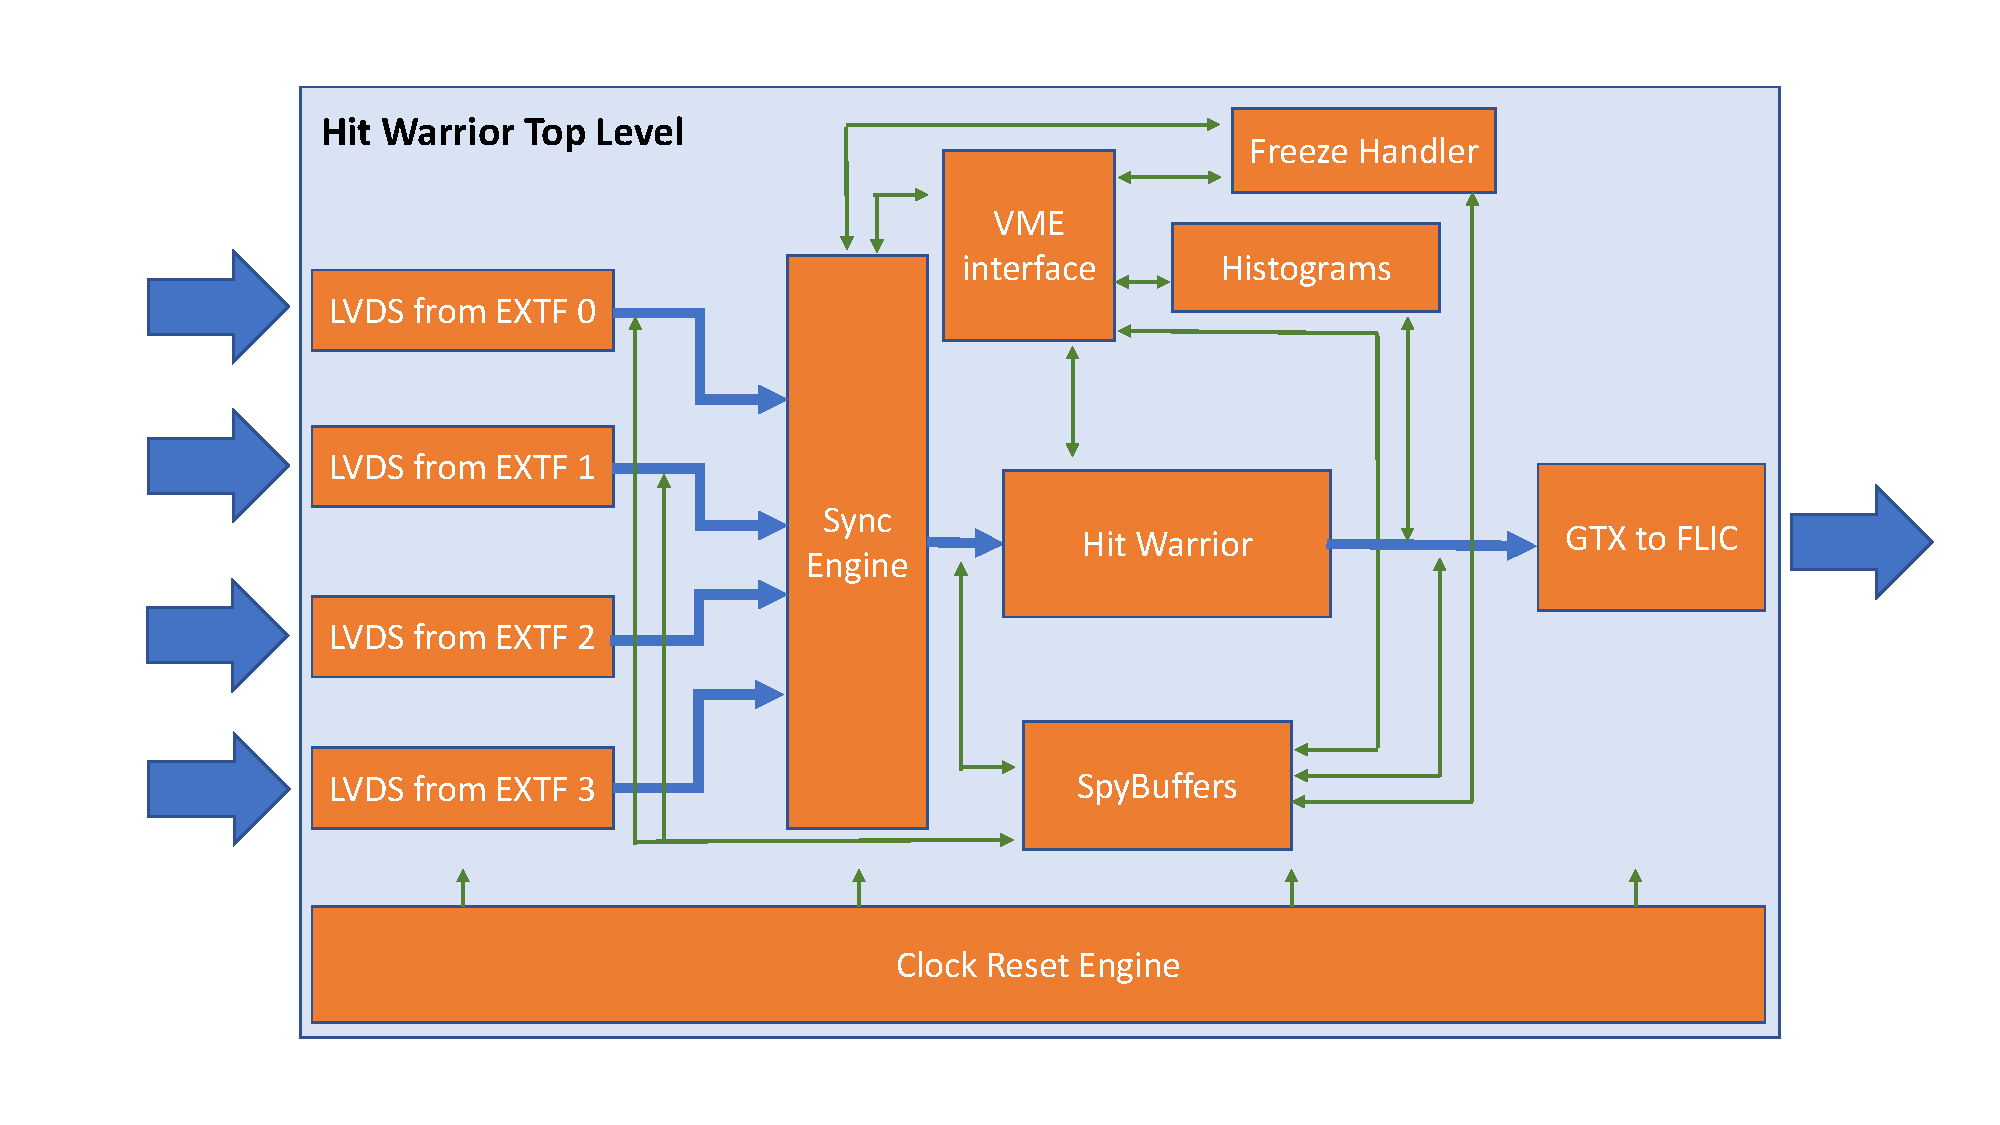
\includegraphics[width=0.75\textwidth]{figures/ftk/hw_top_diagram.pdf}
  \caption{Diagram of the Hit Warrior firmware~\cite{Aad_2021}.}
  \label{fig:hw_top_diagram}
\end{figure}

The Track Parser functions as the first component of the Hit Warrior module, where it examines the data to identify the start of track packets. These packets always start with the keyword ``BDA'' and consist of 28 words. Each track is distributed throughout the FPGA to enable parallel processing of track comparisons. Tracks are processed sequentially, one after another, which makes it practical to use a track counter. The specific processing path for each track depends on this counter. However, the overarching strategy ensures that each new track is compared with all previously received tracks simultaneously. By the time the final track is processed, all necessary track comparisons have been completed.

The first and simplest component to understand in this context is the RAW FIFO (First In, First Out). This acts as an internal storage or buffer for all the tracks corresponding to the current event, storing them in the exact order they were received.
The layout is illustrated in Figure \ref{fig:hw_fifo}.

\begin{figure}[ht]
  \centering
  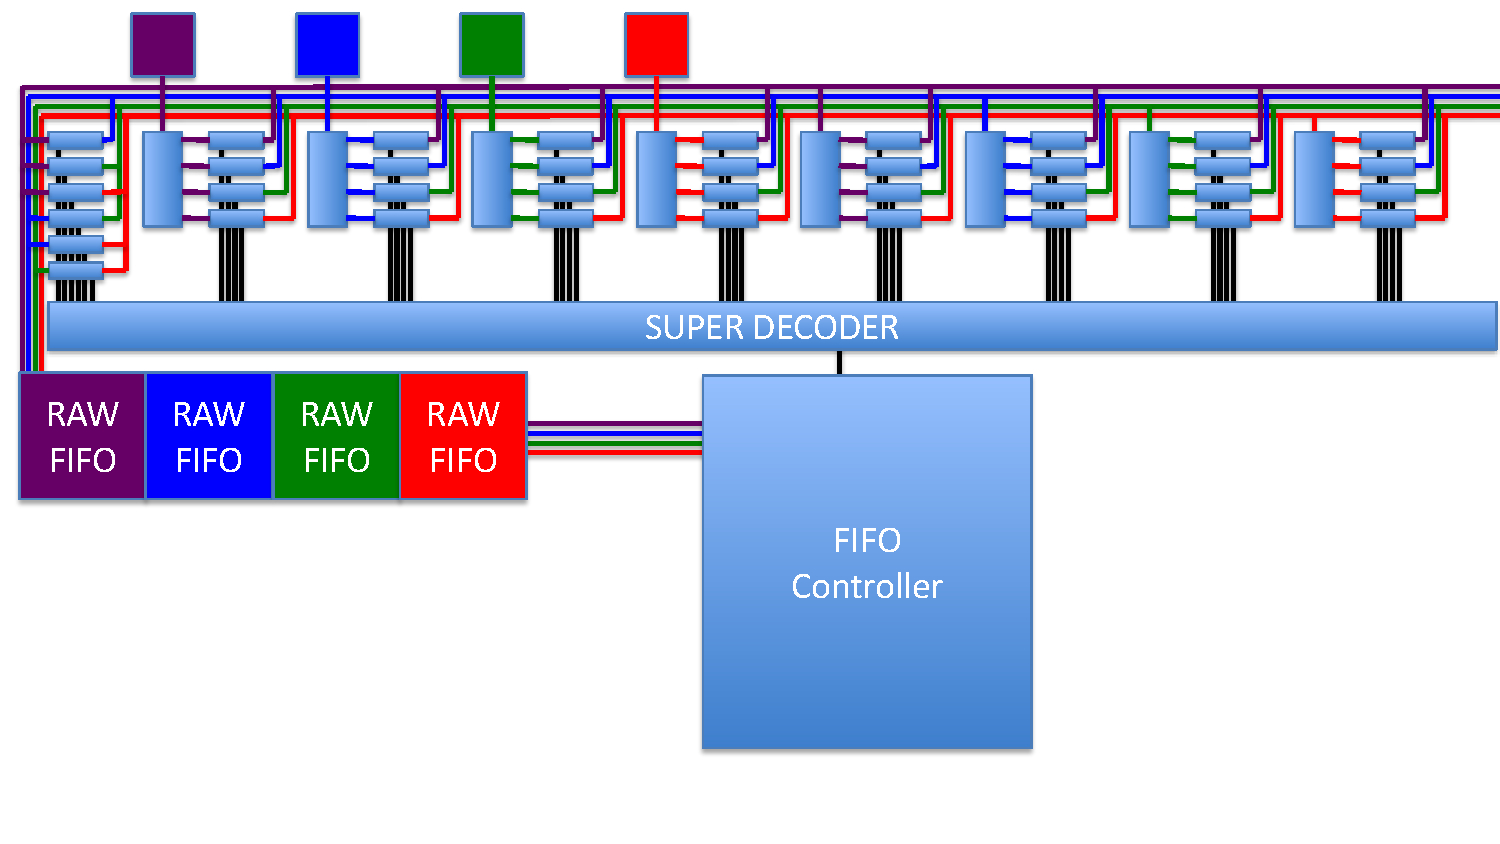
\includegraphics[width=0.75\textwidth]{figures/ftk/hw_fifo.pdf}
  \caption{Hit Warrior FIFO Diagram}
  \label{fig:hw_fifo}
\end{figure}

Tracks are also sent to units called Comparators. The total number of Comparators is limited by available resources, which in turn sets a maximum on the number of tracks that can be effectively compared for an event. Each Comparator is equipped with a small piece of RAM (Random Access Memory) capable of holding a single track packet. Furthermore, each Comparator is directly connected to the stream of incoming tracks, allowing it to receive and compare new track data as it arrives.

%%%Comparators
The comparator conducts comparisons between two tracks on a word-to-word basis to identify matches. Each track packet contains 28 words, comprising 12 for the Track Header and 16 for the hit list. These 16 words are distributed across 12 layers. A match requires at least eight layers to be identical, a criterion determined through simulation to ensure maximum efficiency. For 2D pixel layers, both coordinates must match.

When matches are detected, a selection criterion decides the optimal track. Tracks with the same number of layers are evaluated on their \(\chi^2\) values to select the best one. If the layer count varies, the track with the greater number of layers is chosen. The selection scheme is outlined in the Table~\ref{table:track_selection_scheme}.

\begin{table}[ht]
\centering
\resizebox{0.6\textwidth}{!}{%
\begin{tabular}{ccc}
\hline
\textbf{Track 1} & \textbf{Track 2} & \textbf{Decision} \\
\hline
Nominal & Nominal & Select Track with lowest \(\chi^2\) \\
Nominal & Majority & Select Nominal Track \\
Majority & Majority & Select Track with lowest \(\chi^2\) \\
\hline
\end{tabular}%
}
\caption{Selection scheme for matching tracks.}
\label{table:track_selection_scheme}
\end{table}

After each track is compared, the outcome is forwarded to the Decoder, which logs the results of all track comparisons. Each comparator can issue one of four possible outcomes, encoded as two bits: \textit{idle}, \textit{no match}, \textit{delete RAM}, and \textit{delete Stream}. The Decoder synthesizes these outcomes with the current track count and the comparator's index to generate a "copy vector." This vector is essential for managing the write process to the CUT FIFO.

Once every track for the event has been examined and the copy vector is complete, the RAW FIFO's content is moved. This FIFO contains a copy of every track. This data is then transferred to a second FIFO, named the CUT FIFO, guided by the copy vector to ensure only the valid tracks are preserved. This arrangement allows for the removal of gaps in the data by excluding the tracks as dictated by the copy vector.

\begin{table}[ht]
\centering
\begin{tabular}{ll}
\hline
\textbf{Comparator Output} & \textbf{Meaning} \\
\hline
Idle & No operation \\
No Match & No duplicate found \\
Delete RAM & Remove track from RAM \\
Delete Stream & Remove track from incoming stream \\
\hline
\end{tabular}
\caption{Comparator Results and Their Meanings}
\label{table:comparator_results}
\end{table}

The CUT FIFO then serves as the final repository for the processed tracks, ensuring that only the relevant tracks are stored for further processing.
The decoder, using comparator flags, the index number of each comparator, and the track counter, identifies tracks for deletion. For instance, comparator M can only eliminate track M stored in its RAM or the track currently indexed by the track counter. Each processed track is compared in parallel to all prior ones. In each comparison round, any previous track might be marked for deletion by the incoming track. After each round, the decoder updates the copy vector to record any tracks flagged for removal. When the last track of the event has been compared, the final version of the copy vector is used to regulate the transfer of data from the RAW FIFO to the CUT FIFO, ensuring only the required tracks are retained.

It became apparent later in development that the prototype Hit Warrior firmware couldn’t keep up with the required processing speed. To address this, the system was adapted to process multiple streams in parallel. The Parallel Hit Warrior operates much like the original but at quadruple the speed by handling four streams simultaneously. This choice is aligned with the four EXTF FPGAs on each SSB. Therefore four tracks are inputted into four separate comparators. These comparators have been adapted to match a track in RAM against four incoming stream tracks at the same time. Additionally, a new component, the Cross Comparator, was introduced to compare all six pairings among the four stream tracks.
The layout of the Parallel Hit Warrior is shown in Figure \ref{fig:hw_layout}, and the details of the comparator are revealed in Figure \ref{fig:hw_details}.

\begin{figure}[ht]
  \centering
  \begin{subfigure}[b]{0.5\textwidth}
    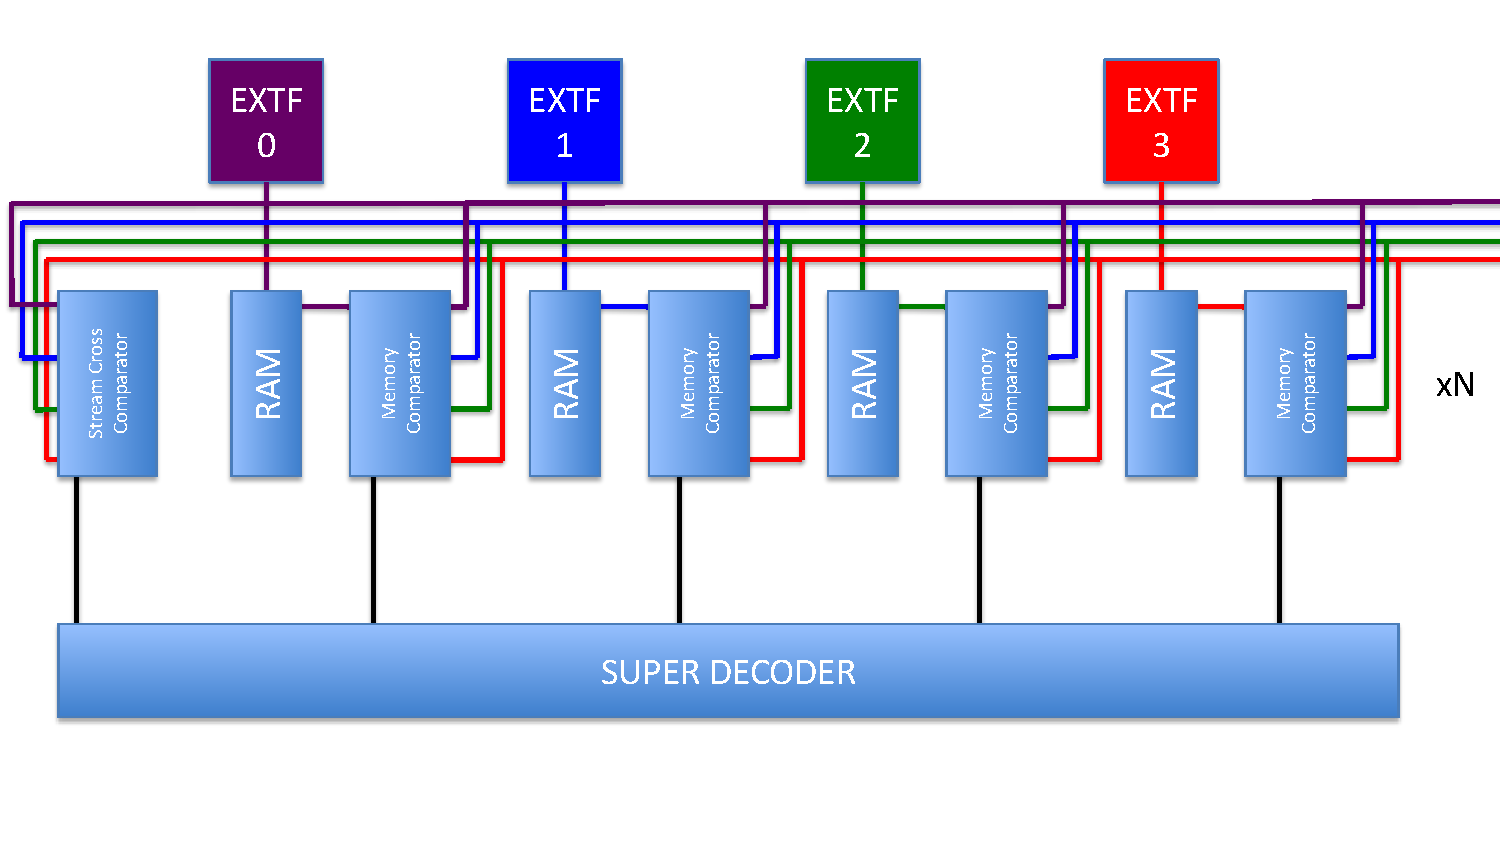
\includegraphics[width=\textwidth]{figures/ftk/hw_layout.pdf}
    \caption{Hit Warrior Layout}
    \label{fig:hw_layout}
  \end{subfigure}%
  \hfill
  \begin{subfigure}[b]{0.5\textwidth}
    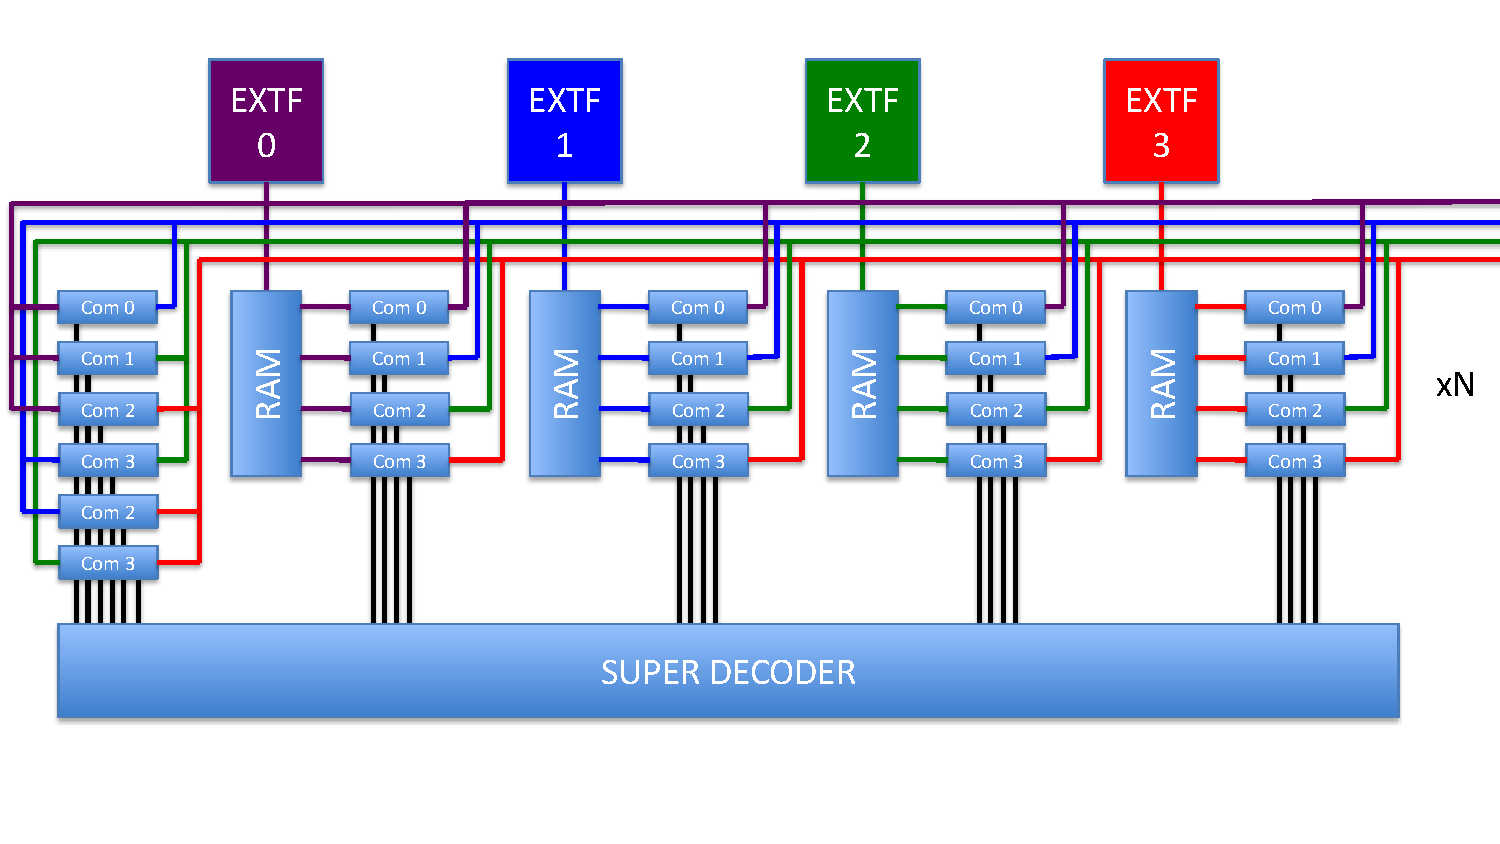
\includegraphics[width=\textwidth]{figures/ftk/hw_details.pdf}
    \caption{Hit Warrior Details}
    \label{fig:hw_details}
  \end{subfigure}
  \caption{Hit Warrior System Components}
  \label{fig:hit_warrior}
\end{figure}

%Spybuffer
The firmware design for the HitWarrior FPGA utilizes circular buffers, known as Spy Buffers, to capture data as it moves through the system, alongside the capability to read out monitoring registers. It also allows for the freezing of monitoring data in the event of errors to aid in debugging. Furthermore, these buffers store synchronized monitoring information and compile histograms of monitoring data. While this firmware design is broadly applied across various components of the FTK system, including the design of synchronization blocks, the SSB version is tailored for the HitWarrior FPGA to meet specific design needs and to accommodate the architecture of the FPGA chip.
As shown in Figure~\ref{fig:hw_top_diagram}, the Spy Buffers monitor the four parallel streams from the EXTF FPGAs, and the output of the Hit Warrior module before sending it to the FLIC.

%my job

My role in the development of the SSB involved updating the firmware for the Hit Warrior FPGA, focusing on parallelizing the prototype Hit Warrior firmware and implementing the Spy Buffers. 
I was deeply involved, often as the sole representative for the SSB, in its commissioning and integration into the ATLAS trigger system. This required extensive hours in the ATLAS control rooms and the underground facilities where the FTK system is installed.



























